\subsection{积分的性质}

规则函数积分的性质，不过是把第一章中已经证明的导数性质翻译成适当的记号而已。

首先，公式 (3) 表明，无论点 \(x, y, z\) 是 \(I\) 中怎样的点，均有

\[
\int_ {x} ^ {x} \mathbf {f} (t) d t = 0\tag{4}
\]

\[
\int_ {x} ^ {y} \mathbf {f} (t) d t + \int_ {y} ^ {x} \mathbf {f} (t) d t = 0\tag{5}
\]

\[
\int_ {x} ^ {y} \mathbf {f} (t) d t + \int_ {y} ^ {z} \mathbf {f} (t) d t + \int_ {z} ^ {x} \mathbf {f} (t) d t = 0\tag{6}
\]

由 II, p.~52 的命题 1，有

\[
\int_ {x _ {0}} (\mathbf {f} + \mathbf {g}) = \int_ {x _ {0}} \mathbf {f} + \int_ {x _ {0}} \mathbf {g}\tag{7}
\]

而且对每个数量 \(k\)

\[
\int_ {x _ {0}} k \mathbf {f} = k \int_ {x _ {0}} \mathbf {f}.\tag{8}
\]

设 \(E, F\) 是 \(\mathbf{R}\) 上的两个完备赋范空间，\(\mathbf{u}\) 是 \(E\) 到 \(F\) 中的连续线性映射。若 \(\mathbf{f}\) 是 \(I\) 上的规则函数且取值于 \(E\)，则 \(\mathbf{u} \circ \mathbf{f}\) 是 \(I\) 上的规则函数且取值于 \(F\)（II, p.~6, 推论 2），并且对 \(a, b \in I\) 有（I, p.~13, 命题 2）

\[
\int_ {a} ^ {b} \mathbf {u} (\mathbf {f} (t)) d t = \mathbf {u} \left(\int_ {a} ^ {b} \mathbf {f} (t) d t\right).\tag{9}
\]

现在设 E, F, G 是 R 上的三个完备赋范空间，\((\mathbf{x}, \mathbf{y}) \mapsto [\mathbf{x} \cdot \mathbf{y}]\) 是 \(E \times F\) 到 G 中的连续双线性映射。设 f 与 g 是定义在 I 上且连续的两个向量函数，分别取值于 E 与 F 中；再假设 f 与 g 是两个规则函数的原函数，我们（滥用语言的说法）把它们记作 \(f'\) 与 \(g'\)（除了在一个可数集的余集上之外，实际上并不能保证这些函数分别等于 f 与 g 的导数）。由 I, p.~6 的命题 3，函数 \(\mathbf{h}(x) = [\mathbf{f}(x) \cdot \mathbf{g}(x)]\) 在 I 的一个可数子集的余集的每一点处都有导数，等于 \([\mathbf{f}(x) \cdot \mathbf{g}'(x)] + [\mathbf{f}'(x) \cdot \mathbf{g}(x)]\)。又，由 {[}x.y{]} 的连续性及 II, p.~55 的推论 2，函数 \([f \cdot g']\) 与 \([f' \cdot g]\) 中的每一个都是 I 上的规则函数；于是有公式

\[
\int_ {a} ^ {b} [ \mathbf {f} ^ {\prime} (t). \mathbf {g} (t) ] d t = [ \mathbf {f} (t). \mathbf {g} (t) ] \big | _ {a} ^ {b} - \int_ {a} ^ {b} [ \mathbf {f} (t). \mathbf {g} ^ {\prime} (t) ] d t\tag{10}
\]

它称为分部积分公式，使我们能求出许多原函数。

例如，分部积分公式给出下面的公式

\[
\int_ {x _ {0}} ^ {x} t \mathbf {f} ^ {\prime} (t) d t = t \mathbf {f} (t) \Big | _ {x _ {0}} ^ {x} - \int_ {x _ {0}} ^ {x} \mathbf {f} (t) d t
\]

从而把函数 \(\mathbf{f}(x)\) 与 \(x\mathbf{f}'(x)\) 两者之一的原函数的计算化为另一个的原函数的计算。

同样，若 \(\mathbf{f}\) 与 \(\mathbf{g}\) 在区间 I 上 \(n\) 次可导，且 \(\mathbf{f}^{(n)}\) 与 \(\mathbf{g}^{(n)}\) 是 I 上的规则函数，则 I, p.~21 的公式 (5) 等价于下式：

\[
\begin{array}{l} \int_ {a} ^ {b} [ \mathbf {f} ^ {(n)} (t). \mathbf {g} (t) ] d t \\ = \left. \left(\sum_ {p = 0} ^ {n - 1} (- 1) ^ {p} [ \mathbf {f} ^ {(n - p - 1)} (t). \mathbf {g} ^ {(p)} (t) ]\right) \right| _ {a} ^ {b} + (- 1) ^ {n} \int_ {a} ^ {b} [ \mathbf {f} (t). \mathbf {g} ^ {(n)} (t) ] d t \end{array}\tag{11}
\]

我们把它称为 n 阶分部积分公式。

现在来翻译复合函数的求导公式（I, p.~9, 命题 5）。设 \(f\) 是定义在 I 上且连续的实函数，它是 I 上某个规则函数的原函数（我们仍（滥用语言的说法）把它记作 \(f'\)）；再设 \(\mathbf{g}\) 是包含 \(f(\mathrm{I})\) 的某个开区间 J 上的连续向量函数（取值于完备赋范空间）；若 \(\mathbf{h}\) 表示 \(\mathbf{g}\) 在 J 上的任意一个原函数，则 \(\mathbf{h}\) 在 J 的每一点处有导数，等于 \(\mathbf{g}\)（II, p.~56, 命题 3）；于是复合函数 \(\mathbf{h} \circ f\) 在 I 的一个可数子集（相对于 I）的余集的所有点处有导数，等于 \(\mathbf{g}(f(x))f'(x)\)（I, p.~9, 命题 5）；由于函数 \(\mathbf{g}(f(x))f'(x)\) 是规则的（II, p.~55, 推论 2），我们可以写出公式

\[
\int_ {a} ^ {b} \mathbf {g} (f (t)) f ^ {\prime} (t) d t = \int_ {f (a)} ^ {f (b)} \mathbf {g} (u) d u\tag{12}
\]

它称为变量替换公式，同样有助于原函数的计算。

例如，若取 \(f(x) = x^{2}\)，则可见公式 (12) 把函数 \(\mathbf{g}(x)\) 与 \(x\mathbf{g}(x^{2})\) 的原函数的计算由其中一个化为另一个。

为了把中值定理（I, p.~14, 定理 1）翻译到实规则函数的原函数上，我们首先注意，紧区间 I 上的实规则函数 \(f\) 在 I 上有界；设 J 是 I 中使 \(f\) 连续的点所成的集，并令 \(m = \inf_{x \in \mathrm{J}} f(x)\)，\(\mathrm{M} = \sup_{x \in \mathrm{J}} f(x)\)；我们知道（II, p.~54, 定理 3）\(\mathrm{I} \cap \complement \mathrm{J}\) 是可数的；此外，若 B 是 I 的任意可数子集相对于 I 的余集，且 \(m' = \inf_{x \in \mathrm{B}} f(x)\)，\(\mathrm{M}' = \sup_{x \in \mathrm{B}} f(x)\)，则有 \(m' \leqslant m \leqslant M \leqslant M'\)：事实上，对每一点 \(x \in J\)，都存在 B 中任意接近 x 的点 y，于是 \(m' \leqslant f(y) \leqslant M'\)；由于 f 在点 x 连续，令 y 趋于 x（y 保持属于 B）便得 \(m' \leqslant f(x) \leqslant M'\)，这就证明了我们的断言。这样，把中值定理翻译过来便得下列命题：

命题 6（中值定理）。设 \(f\) 是紧区间 \(\mathrm{I} = [a, b]\) 上的实规则函数；若 \(\mathrm{J}\) 是 \(\mathrm{I}\) 中使 \(f\) 连续的点所成的集，且 \(m = \inf_{x \in \mathrm{J}} f(x)\)，\(\mathrm{M} = \sup_{x \in \mathrm{J}} f(x)\)，则

\[
m <   \frac {1}{b - a} \int_ {a} ^ {b} \mathbf {f} (t) d t <   \mathbf {M}\tag{13}
\]

除非 \(f\) 在 \(\mathbf{J}\) 上取常值，此时 (13) 的三项相等。

换言之，规则函数 \(f\) 在 I 中的平均值介于 \(f\) 在 I 中使 \(f\) 连续的子集上的各界之间。

推论 1. 若一个实规则函数 \(f\) 在 \(I\) 上使得 \(f(x) \geqslant 0\)（在 \(f\) 连续的各点处），则 \(\frac{1}{b - a} \int_{a}^{b} f(t) dt > 0\)，除非 \(f(x) = 0\)（在 \(f\) 连续的各点处）。

推论 2. 设 f 与 g 是 I 上的两个实规则函数，使得在 g 连续的各点处 \(g(x) \geqslant 0\)；若 m 与 M 是 f 在使 f 连续的点所成之集上的下确界与上确界，则

\[
\frac {m}{b - a} \int_ {a} ^ {b} g (t) d t \leqslant \frac {1}{b - a} \int_ {a} ^ {b} f (t) g (t) d t \leqslant \frac {\mathrm{M}}{b - a} \int_ {a} ^ {b} g (t) d t.\tag{14}
\]

除非 \(g(x)(f(x) - m) = 0\)（相应地，\(g(x)(f(x) - \mathbf{M}) = 0\)）在 \(f\) 与 \(g\) 连续的每一点处成立，否则前两项（相应地，后两项）不相等。

对向量函数，中值定理（I, p.~15, 定理 2）给出下列命题：

命题 7. 设 \(\mathbf{f}\) 是紧区间 \(\mathrm{I} = [a, b]\) 上的规则向量函数，取值于完备赋范空间 \(\mathrm{E}\)，并设 \(g\) 是 \(\mathrm{I}\) 上的实规则函数，使得 \(g(x) \geqslant 0\) 在 \(g\) 连续的各点处成立；在这些条件下

\[
\left\| \int_ {a} ^ {b} \mathbf {f} (t) g (t) d t \right\| \leqslant \int_ {a} ^ {b} \| \mathbf {f} (t) \| g (t) d t.\tag{15}
\]

特别地，

\[
\left\| \int_ {a} ^ {b} \mathbf {f} (t) d t \right\| \leqslant \int_ {a} ^ {b} \| \mathbf {f} (t) \| d t.\tag{16}
\]

\subsection{泰勒公式余项的积分公式；高阶原函数}

n 阶分部积分公式（II, p.~60, 公式 (11)）使我们可以把余项 \(\mathbf{r}_{n}(x)\)——即一个在区间 I 上具有规则的 \((n+1)^{th}\) 导数的函数的 n 阶泰勒展开中的余项——用一个积分表出（I, p.~22）；事实上，在 (12) 中把 f 换成 \(f'\)、b 换成 x、\(g(t)\) 换成函数 \((t-x)^{n}/n!\)，即得

\[
\begin{array}{l} \mathbf {f} (x) = \mathbf {f} (a) + \mathbf {f} ^ {\prime} (a) \frac {(x - a)}{1 !} + \mathbf {f} ^ {\prime \prime} (a) \frac {(x - a) ^ {2}}{2 !} + \dots \\ \qquad + \mathbf {f} ^ {(n)} (a) \frac {(x - a) ^ {n}}{n !} + \int_ {a} ^ {x} \mathbf {f} ^ {(n + 1)} (t) \frac {(x - t) ^ {n}}{n !} d t \end{array}\tag{17}
\]

换言之

\[
\mathbf {r} _ {n} (x) = \int_ {a} ^ {x} \mathbf {f} ^ {(n + 1)} (t) \frac {(x - t) ^ {n}}{n !} d t,\tag{18}
\]

这个公式常使我们能得到余项的简单界。

给定区间 I 上的一个规则函数 f，f 的任意一个原函数 g 在 I 上连续，从而自身又有原函数；f 的任意原函数的任意原函数称为 f 的二阶原函数。更一般地，f 的 n - 1 阶原函数的一个原函数称为 f 的 n 阶原函数。对 n 用归纳法立即看出，f 的两个 n 阶原函数之差是一个次数至多等于 n - 1 的多项式（系数在 E 中）。若给定了 f 的一个 n 阶原函数在一点 \(a \in I\) 处的值及其前 n - 1 阶导数在该点的值，它就完全确定了。

特别地，\(\int_{a}^{(n)}\mathbf{f}\) 表示 \(n\) 阶原函数（指 \(\mathbf{f}\) 的）中连同其前 \(n - 1\) 阶导数在点 \(a\) 处一同为零的那一个。把 \(n - 1\) 阶泰勒公式应用于这个原函数就表明：若 \(\mathbf{g} = \int_{a}^{(n)}\mathbf{f}\)，则

\[
\mathbf {g} (x) = \int_ {a} ^ {x} \mathbf {f} (t) \frac {(x - t) ^ {n - 1}}{(n - 1) !} d t\tag{19}
\]

从而把 n 阶原函数的确定化为单独一个积分。

\section{非紧区间上的积分}

\subsection{非紧区间上积分的定义}

设 I 是紧区间 \([a, b]\)，含于扩充实直线 \(\overline{R}\)（a 与 b 可以是无穷）；设 f 是定义在 {]}a, b{[} 上、取值于 R 上的完备赋范空间 E 中的函数。把 II, p.~51 的定义 1 加以推广，我们说：定义在 \([a, b]\) 上且取值于 E 中的函数 g 是 f 的原函数，如果它在 \([a, b]\) 上连续（特别是在端点 a 与 b 处连续），并且在这区间的一个可数子集的余集的各点处具有等于 \(\mathbf{f}(x)\) 的导数（余集相对于 {]}a, b{[} 取）。

我们将限于如下情形：存在一个有限的严格递增序列 \((c_i)_{0\leqslant i\leqslant n}\)，由 \(\mathrm{I} = [a,b]\) 的点组成，使得 \(c_0 = a\)、\(c_n = b\)，并且使得 \(\mathbf{f}\) 在每个开区间 \(]c_i\) , \(c_{i + 1}[\) 上是规则的，尽管在包含至少一个点 \(c_i\)（作为 \(\mathrm{I}\) 的内点）的每个开区间上不一定都是规则的；这样的函数称为 \(]a\) , \(b[\) 上的分段规则函数。我们注意，\(]a\) , \(b[\) 上的规则函数是分段规则的（在前面的定义中取 \(n = 1\)）。

若 \(\mathbf{f}\)（按上面明确的意义）有一个原函数 \(\mathbf{g}\)，且若 \(c\) 是区间 \([c_i, c_{i+1}[(0 \leqslant i \leqslant n-1)\) 中的一点，则据假设，对此区间中的每个 \(x\)，有 \(\mathbf{g}(x) - \mathbf{g}(c) = \int_c^x \mathbf{f}(t) dt\)；由于 \(\mathbf{g}\) 据假设在 I 上连续，可见 \(\int_c^x \mathbf{f}(t) dt\) 当 \(x\) 从右边趋于 \(c_i\) 时以及当 \(x\) 从左边趋于 \(c_{i+1}\) 时在 E 中趋于一个极限。反之，假设这些条件对一切 \(t\) 都满足，并设 \(\mathbf{g}_i\) 是 \(\mathbf{f}\) 在区间 \([c_i, c_{i+1}[(0 \leqslant i \leqslant n-1)\) 上的一个原函数；我们立即注意到：函数 \(\mathbf{g}\) 在诸点 \(c_i\) 所成之集相对于 I 的余集上按如下条件定义：它等于 \(\mathbf{g}_i(x) + \sum_{k=1}^i (\mathbf{g}_{k-1}(c_k-) - \mathbf{g}_k(c_k+))\)（在 \([c_i, c_{i+1}[\) 上，对 \(0 \leqslant i \leqslant n-1\)）；它在 I 的每个异于诸 \(c_i\) 的点处连续，并且在每个这样的点处有极限；因此它可以连续地延拓到每个这样的点，而延拓所得的函数显然是 \(\mathbf{f}\) 在 I 上的一个原函数。此外显然，\(\mathbf{f}\) 的任何其他原函数都具有形式 \(\mathbf{g} + \mathbf{a}\)（\(\mathbf{a}\) 是 E 的一个元素）。

定义 1. 我们说向量函数 \(\mathbf{f}\)（在区间 \(]a\) , \(b[\)（属于 \(\overline{\mathbf{R}}\)）上分段规则的）在这个区间上有一个积分，如果 \(\mathbf{f}\) 在 \([a, b]\) 上有一个原函数；若 \(\mathbf{g}\) 是 \(\mathbf{f}\) 在 \([a, b]\) 上的任一原函数，且 \(x_0\) 与 \(x\) 是 \([a, b]\) 上的任意两点，则称元素 \(\mathbf{g}(x) - \mathbf{g}(x_0)\) 为 \(\mathbf{f}\) 从 \(x_0\) 到 \(x\) 的积分，并记作 \(\int_{x_0}^x \mathbf{f}(t) dt\)。

当区间 \([x_0, x]\) 不含任何点 \(c_i\) 时，这个概念显然与此前所定义的概念一致。

定义 1 之前的这些注记表明，为使 \(\mathbf{f}\) 在 \(]a\) , \(b[\) 上有一个积分，必须且只需它在每个区间 \([c_i, c_{i+1}]\) 上的限制在该区间上有一个积分。换言之，可以化归为如下的情形：\(\mathbf{f}\) 在非紧区间 \(\mathrm{I} \subset \mathbf{R}\) 上是规则的，其端点为 \(a, b\)（\(a < b\)），并且：\(1^\circ\) 数 \(a, b\) 中（至少）有一个是无穷的；\(2^\circ\) 或者 \(\mathbf{f}\) 在包含点 \(a, b\) 中至少一个的每个紧区间上不是规则的（这两个假设并不互斥）。为使 \(\mathbf{f}\) 在 \(\mathrm{I}\) 上有一个积分，必须且只需积分 \(\int_x^y \mathbf{f}(t) dt\) 当点 \((x, y)\) 趋于 \((a, b) \in \overline{\mathbf{R}}^2\) 而保持属于 \(\mathrm{I} \times \mathrm{I}\) 时趋于一个极限：而这个极限不是别的，正是依定义 1 的 \(\int_a^b \mathbf{f}(t) dt\)。滥用语言的说法，人们不说 \(\mathbf{f}\) 在 \(\mathrm{I}\) 上有一个积分，而说积分 \(\int_a^b \mathbf{f}(t) dt\) 是收敛的（或收敛）。

例。1) 积分 \(\int_{1}^{+\infty} dt / t^{2}\) 收敛且等于 1，因为

\[
\int_ {1} ^ {x} \frac {d t}{t ^ {2}} = 1 - \frac {1}{x}.
\]

\begin{enumerate}
\def\labelenumi{\arabic{enumi})}
\setcounter{enumi}{1}
\tightlist
\item
  积分 \(\int_0^1 dt / \sqrt{t}\) 收敛且等于 2，因为
\end{enumerate}

\[
\int_ {x} ^ {1} \frac {d t}{\sqrt {t}} = 2 (1 - \sqrt {x}) \quad \text { for } \quad x > 0.
\]

\begin{enumerate}
\def\labelenumi{\arabic{enumi})}
\setcounter{enumi}{2}
\tightlist
\item
  设 \((\mathbf{u}_n)_{n\geqslant 1}\) 是 E 的点的一个无穷序列，\(\mathbf{f}\) 是由下列条件定义在区间 {[}1, \(+\infty[\) 上的阶梯函数：\(\mathbf{f}(x) = \mathbf{u}_n\)（当 \(n\leqslant x < n + 1\)）。那么，为使积分 \(\int_1^{+\infty}\mathbf{f}(t)dt\) 收敛，必须且只需通项为 \(\mathbf{u}_n\) 的级数在 E 中收敛；事实上，有
\end{enumerate}

\[
\int_ {1} ^ {n} \mathbf {f} (t) d t = \sum_ {p = 1} ^ {n - 1} \mathbf {u} _ {p},
\]

故条件是必要的；反之，若通项为 \(\mathbf{u}_n\) 的级数在 E 中收敛，则 \(\lim_{n\to \infty}\mathbf{u}_n = 0\)；而今若 \(n\leqslant x\leqslant n + 1\)，就有 \(\int_1^n\mathbf{f}(t)dt = \sum_{p = 1}^{n - 1}\mathbf{u}_p +\) \(\mathbf{u}_n(x - n)\)，故这个积分具有极限 \(\sum_{n = 1}^{\infty}\mathbf{u}_n\)（当 \(x\) 趋于 \(+\infty\) 时）。

立即可以看出，若分段规则函数 \(\mathbf{f}\) 在 I 上有一个积分，则 II, p.~59 的公式 (4) 至 (9) 仍然有效。类似地，II, p.~59 的公式 (10) 按如下方式推广：假设 \(\mathbf{f}\) 与 \(\mathbf{g}\) 是规则函数 \(\mathbf{f}'\) 与 \(\mathbf{g}'\) 在 \(]a\) , \(b[\) 上的原函数，并用 \([\mathbf{f}.\mathbf{g}]|_a^b\) 表示 \([\mathbf{f}.\mathbf{g}]|_x^y\) 当 \((x, y)\) 趋于 \((a, b)\)（且 \(a < x \leqslant y < b\)）时的极限（如果它存在）；那么，若（三个）表达式 \([\mathbf{f}.\mathbf{g}]|_a^b\)、\(\int_a^b [\mathbf{f}(t).\mathbf{g}'(t)] dt\) 与 \(\int_a^b [\mathbf{f}'(t).\mathbf{g}(t)] dt\) 中有两个有意义，则第三个也有意义，并且 II, p.~59 的公式 (10) 成立。

最后，设 \(f\) 是定义且连续在 \(I = ]a\) , \(b[\) 上的实函数，并且是某个规则函数 \(f'\) 在 \(]a\) , \(b[\) 上的原函数；另一方面，设 \(\mathbf{g}\) 是开区间 \(J\)（包含 \(f(I)\)）上的连续向量函数；若函数 \(\mathbf{g}(f(x))f'(x)\) 在 \(I\) 上有一个积分，且若 \(f\) 在点 \(a\) 与 \(b\) 处趋于一个极限（有限或无穷），则 \(\mathbf{g}\) 有一个从 \(f(a+)\) 到 \(f(b-)\) 的积分，并且有公式

\[
\int_ {a} ^ {b} \mathbf {g} (f (t)) f ^ {\prime} (t) d t = \int_ {f (a +)} ^ {f (b -)} \mathbf {g} (u) d u.\tag{1}
\]

事实上，若 \((x, y)\) 趋于 \((a, b)\)，则据假设 \((f(x), f(y))\) 趋于 \((f(a+), f(b-))\)；只需在 x 与 y 之间应用 II, p.~60 的公式 (12) 并取极限，即得 (1)。

给定非紧区间 \(I \subset R\) 上的一个规则函数 f，其端点为 a 与 b（a \textless{} b），f 在 I 上有积分这一条件可以表述如下。紧区间 \(J \subset I\) 构成一个有向集 \(\mathfrak{K}(I)\)（关于关系 \(\subset^{1}\)），因为若 \([\alpha, \beta]\) 与 \([\gamma, \delta]\) 是含于 I 的两个紧区间，且令 \(\lambda = \min(\alpha, \gamma)\)、\(\mu = \max(\beta, \delta)\)，则区间 \([\lambda, \mu]\) 含于 I 且包含所考虑的两个区间。对每个含于 I 的紧区间 \(J = [\alpha, \beta]\)，令

\[
\int_ {\mathrm{J}} \mathbf {f} (t) d t = \int_ {\alpha} ^ {\beta} \mathbf {f} (t) d t;
\]

为使 f 在 I 上有一个积分，必须且只需映射 \(\mathbf{J} \mapsto \int_{\mathrm{J}} \mathbf{f}(t) dt\) 关于有向集 \(\mathcal{K}(\mathrm{I})\) 有一个极限；这个极限就是积分 \(\int_{a}^{b} \mathbf{f}(t) dt\)，我们仍把它记作 \(\int_{\mathrm{I}} \mathbf{f}(t) dt\)。

命题 1（积分的柯西准则）。设 \(\mathbf{f}\) 是区间 \(\mathrm{I} \subset \mathbf{R}\) 上的规则函数，其端点为 \(a\) 与 \(b\)（\(a < b\)）。为使积分 \(\int_{a}^{b} \mathbf{f}(t) dt\) 存在，必须且只需：对每个 \(\varepsilon > 0\)，存在一个含于 I 的紧区间 \(\mathrm{J}_0 = [\alpha, \beta]\)，使得对任何紧区间 \(\mathrm{K} = [x, y]\)（含于 I 且与 \(\mathrm{J}_0\) 无公共内点），都有 \(\left\| \int_{\mathrm{K}} \mathbf{f}(t) dt \right\| \leqslant \varepsilon\)。

事实上，由于 E 是完备的，柯西准则表明：为使积分 \(\int_{\mathrm{I}} \mathbf{f}(t) dt\) 收敛，必须且只需对任何 \(\varepsilon > 0\) 存在一个紧区间 \(\mathrm{J}_0 = [\alpha, \beta]\)，使得对每个满足 \(\mathrm{J}_0 \subset \mathrm{J} \subset I\) 的紧区间 J，有 \(\left\| \int_{\mathrm{J}} \mathbf{f}(t) dt - \int_{\mathrm{J}_0} \mathbf{f}(t) dt \right\| \leqslant \varepsilon\)。该命题将由下面的引理推出：

引理。设 \(J_{0} = [\alpha, \beta]\) 是含于 I 的紧区间。为使 \(\left\|\int_{J} \mathbf{f}(t) dt - \int_{J'} \mathbf{f}(t) dt\right\| \leqslant \varepsilon\) 对每一对含于 I 且包含 \(J'\) 的紧区间 J、\(J'\) 都成立，必要的是 \(\left\|\int_{K} \mathbf{f}(t) dt\right\| \leqslant \varepsilon\)，而且 \(\left\|\int_{K} \mathbf{f}(t) dt\right\| \leqslant \varepsilon/2\) 就是充分的（对每个含于 I 且与 \(J_{0}\) 无公共内点的紧区间 K）。

事实上，若对 \(J_{0} \subset J \subset I\) 与 \(J_{0} \subset J' \subset I\) 有

\[
\left\| \int_ {J} \mathbf {f} (t) d t - \int_ {J ^ {\prime}} \mathbf {f} (t) d t \right\| \leqslant \varepsilon
\]

则特别地可以看出，对 \(x \leqslant y \leqslant \alpha\)，或对 \(\beta \leqslant x \leqslant y\)（x 与 y 属于 I），有 \(\left\|\int_{x}^{y} \mathbf{f}(t) dt\right\| \leqslant \varepsilon\)。反之，若 \(\left\|\int_{K} \mathbf{f}(t) dt\right\| \leqslant \varepsilon/2\) 对每个紧区间 \(K \subset I\)（满足 \(K \cap J_{0} = \emptyset\)）都成立，且若 \(J = [x, y]\)、\(J' = [z, t]\) 是含于 I 且包含 \(J_{0}\) 的两个紧区间，则有

\[
\left\| \int_ {J} \mathbf {f} (t) d t - \int_ {J ^ {\prime}} \mathbf {f} (t) d t \right\| = \left\| \int_ {x} ^ {z} \mathbf {f} (t) d t + \int_ {t} ^ {y} \mathbf {f} (t) d t \right\| \leqslant \varepsilon ,
\]

因为

\[
x \leqslant \alpha \leqslant \beta \leqslant y \quad \text { and } \quad z \leqslant \alpha \leqslant \beta \leqslant t.
\]

例。若区间 I 有界，且 \(\mathbf{f}\) 在 I 上有界，则积分 \(\int_{\mathrm{I}}\mathbf{f}(t)dt\) 总存在，因为由中值定理，对 \(y\leqslant \alpha \leqslant \beta \leqslant z\) 有

\[
\left\| \int_ {y} ^ {\alpha} \mathbf {f} (t) d t \right\| \leqslant (\alpha - a) \sup _ {x \in I} \| \mathbf {f} (x) \|, \quad \left\| \int_ {\beta} ^ {z} \mathbf {f} (t) d t \right\| \leqslant (b - \beta) \sup _ {x \in I} \| \mathbf {f} (x) \|
\]

只需取 \(\alpha - a\) 与 \(b - \beta\) 足够小，柯西准则便得到满足。可以注意，在这种情形下，f 在 I 上的原函数在 I 的左端点（相应地，右端点）处不一定有右（相应地，左）导数（当该数为有限时），这与 I 紧且 f 在 I 上规则的情形不同（参见 II, p.~33, 习题 1）。

\subsection{非紧区间上正函数的积分}

命题 2. 设 f 是一个 \(\geqslant 0\) 的实规则函数，定义在区间 \(I \subset R\) 上，其端点为 a 与 b（a \textless{} b）。为使积分 \(\int_{a}^{b} f(t) dt\) 存在，必须且只需：当 J 跑遍含于 I 的紧区间所成之集时，数集 \(\int_{J} f(t) dt\) 有上界；此时积分 \(\int_{a}^{b} f(t) dt\) 就是数集 \(\int_{J} f(t) dt\) 的上确界。

事实上，由于 \(f \geqslant 0\)，关系 \(J \subset J'\) 蕴含

\[
\int_ {J} f d t \leqslant \int_ {J ^ {\prime}} f d t;
\]

故映射 \(J \mapsto \int_{J} f dt\) 是递增的，而本命题由单调极限定理（Gen.~Top., IV, p.~349, 定理 2）得出。

当映射 \(J \mapsto \int_{J} f(t) dt\) 无界时，它有极限 \(+\infty\)（关于有向集 \(\mathcal{K}(I)\)）；这时人们（滥用语言的说法）说积分 \(\int_{a}^{b} f(t) dt\) 等于 \(+\infty\)。在 \(n^{\circ} 1\) 中建立的积分的性质（当所涉及的是 \(\geqslant 0\) 的函数时）可以推广到所考虑的某些积分为无穷的情形，只要它们所在的关系式有意义。

命题 3（比较原理）。设 f 与 g 是区间 \(I \subset R\) 上的两个实规则函数，使得在 f 与 g 连续的每一点处 \(0 \leqslant f(x) \leqslant g(x)\)（参见 II, p.~61, 命题 6）。若 g 在 I 上的积分收敛，则 f 的积分也收敛，且有 \(\int_{I} f(t) dt \leqslant \int_{I} g(t) dt\)。此外，除非在 I 中 f 与 g 都连续的每一点处 \(f(x) = g(x)\)，否则这两个积分不可能相等。

现在，对每个紧区间 \(\mathrm{J} \subset \mathrm{I}\) 有

\[
\int_ {J} f (t) d t \leqslant \int_ {J} g (t) d t;
\]

由于 \(\int_{\mathrm{J}} g(t) dt \leqslant \int_{\mathrm{I}} g(t) dt\)，诸积分 \(\int_{\mathrm{J}} f dt\) 有上界，故积分 \(\int_{\mathrm{I}} f(t) dt\) 收敛；而且，取极限便得 \(\int_{\mathrm{I}} f(t) dt \leqslant \int_{\mathrm{I}} g(t) dt\)。再设 \(f(x) < g(x)\) 在一个点 \(x \in \mathrm{I}\) 处成立（在该点 \(f\) 与 \(g\) 连续）；存在一个含于 I、不退化为（单个）点的紧区间 \([c, d]\)，使得 \(x \in [c, d]\)；有 \(\int_{c}^{d} f(t) dt < \int_{c}^{d} g(t) dt\)（II, p.~61, 推论 1），又因由上面所述有 \(\int_{a}^{c} f(t) dt \leqslant \int_{a}^{c} g(t) dt\) 与 \(\int_{d}^{b} f(t) dt \leqslant \int_{d}^{b} g(t) dt\)，逐项相加便得 \(\int_{a}^{b} f(t) dt < \int_{a}^{b} g(t) dt\)。

本命题提供了判定函数 \(f \geqslant 0\) 的积分收敛与否的最常用手段，即：把 \(f\) 与一个较简单的函数 \(g \geqslant 0\) 相比较，后者的积分是否收敛已经是知道的；在第五章中我们将看到，在最常见的情形中如何寻找比较函数；并由此外推出积分与级数收敛的常用判别法。

\subsection{绝对收敛积分}

定义 2. 我们说规则函数 \(\mathbf{f}\) 在区间 \(\mathrm{I} \subset \mathbf{R}\) 上的积分是绝对收敛的，如果正函数 \(\| \mathbf{f}(x) \|\) 的积分收敛。

命题 4. 若 \(\mathbf{f}\) 在 \(\mathrm{I}\) 上的积分绝对收敛，则它收敛，且有

\[
\left\| \int_ {I} \mathbf {f} (t) d t \right\| \leqslant \int_ {I} \| \mathbf {f} (t) \| d t.\tag{2}
\]

事实上，对每个紧区间 \(J \subset I\) 有（II, p.~61, 公式 (16)）

\[
\left\| \int_ {J} \mathbf {f} (t) d t \right\| \leqslant \int_ {J} \| \mathbf {f} (t) \| d t.\tag{3}
\]

若正函数 \(\|\mathbf{f}(x)\|\) 的积分收敛，则对每个 \(\varepsilon > 0\) 存在一个含于 I 的紧区间 \([\alpha, \beta]\)，使得对每个紧区间 \([x, y]\)（含于 I 且与 \([\alpha, \beta]\) 无公共内点），有 \(\int_{x}^{y} \|\mathbf{f}(t) dt\| \leqslant \varepsilon\)（II, p.~65, 命题 1）；由此推出 \(\left\|\int_{x}^{y} \mathbf{f}(t) dt\right\| \leqslant \varepsilon\)，这表明 I 上的积分收敛（II, p.~16, 命题 1）；在 (3) 中取极限便得不等式 (2)。

推论。设 E, F, G 是 R 上的三个完备赋范空间，\((\mathbf{x}, \mathbf{y}) \mapsto [\mathbf{x}, \mathbf{y}]\) 是 \(E \times F\) 到 G 中的连续双线性映射。设 f, g 是 I 上的两个规则函数，分别取值于 E 与 F 中。若 f 在 I 上有界且 \(\mathbf{g}\) 的积分在 I 上绝对收敛，则 \([\mathbf{f},\mathbf{g}]\) 的积分绝对收敛。

事实上，存在一个数 \(h > 0\)，使得 \(\| [\mathbf{x},\mathbf{y}] \| \leqslant h \| \mathbf{x} \|\) . \(\| \mathbf{y} \|\) 恒成立（Gen.~Top., IX, p.~173, 定理 1）；若令 \(k = \sup_{x \in I} \| \mathbf{f}(x) \|\)，则在 I 上有 \(\| [\mathbf{f}(x),\mathbf{g}(x)] \| \leqslant hk \| \mathbf{g}(x) \|\)；于是比较原理表明 {[}f,g{]} 的积分绝对收敛，且由 (2)，

\[
\left\| \int_ {I} [ \mathbf {f} (t). \mathbf {g} (t) ] d t \right\| \leqslant h k \int_ {I} \| \mathbf {g} (t) \| d t.
\]

注记。一个积分可以收敛而非绝对收敛；II, p.~64 的例 3 就表明了这一点，那里通项为 \(u_{n}\) 的级数收敛而非绝对收敛。

\section{依赖于参数的函数的导数与积分}

\subsection{紧区间上函数列极限的积分}

把 II, p.~52 的定理 1 应用于紧区间上规则函数这一特殊情形，用积分的适当记号翻译出来就是：

命题 1. 设 A 是被一个滤子 \(\mathfrak{F}\) 所滤化的集合，\((\mathbf{f}_{\alpha})_{\alpha \in \mathrm{A}}\) 是紧区间 \(\mathrm{I} = [a, b]\) 上的一个规则函数族；若函数 \(\mathbf{f}_{\alpha}\) 在 I 上一致收敛于一个（规则的）函数 \(\mathbf{f}\)（关于滤子 \(\mathfrak{F}\)），则

\[
\lim _ {\mathfrak {F}} \int_ {a} ^ {b} \mathbf {f} _ {\alpha} (t) d t = \int_ {a} ^ {b} \mathbf {f} (t) d t.\tag{1}
\]

这个命题的两个推论在应用中很重要：

推论 1. 设 \((\mathbf{f}_n)\) 是紧区间 \(\mathrm{I} = [a, b]\) 上的一个规则函数序列。若序列 \((\mathbf{f}_n)\) 在 \(\mathrm{I}\) 上一致收敛于一个（规则的）函数 \(\mathbf{f}\)，则有

\[
\lim _ {n \rightarrow \infty} \int_ {a} ^ {b} \mathbf {f} _ {n} (t) d t = \int_ {a} ^ {b} \mathbf {f} (t) d t.\tag{2}
\]

特别地，若一个级数，其通项 \(u_{n}\) 是 I 上的规则函数，在 I 上一致收敛于 f，则以 \(\int_{a}^{b}\mathbf{u}_{n}(t)dt\) 为通项的级数收敛且其和为 \(\int_{a}^{b}\mathbf{f}(t)dt\)（“一致收敛级数的逐项积分”）。

推论 2. 设 A 是拓扑空间 F 的一个子集，f 是 I × A 到 R 上的完备赋范空间 E 中的一个映射，使得对每个 \(\alpha \in A\)，函数 \(x \mapsto \mathbf{f}(x, \alpha)\) 在 I 上是规则的。若函数 \(x \mapsto \mathbf{f}(x, \alpha)\) 在 I 上一致收敛于一个（规则的）函数 \(x \mapsto \mathbf{g}(x)\)（当 \(\alpha\) 趋于一点 \(\alpha_{0} \in \overline{A}\) 而保持属于 A 时），则有

\[
\lim _ {\alpha \rightarrow \alpha_ {0}, \alpha \in \mathrm{A}} \int_ {a} ^ {b} \mathbf {f} (x, \alpha) d x = \int_ {a} ^ {b} \mathbf {g} (x) d x.\tag{3}
\]

特别地：

命题 2（“积分对参数的连续性”）。设 F 是紧空间，I = {[}a, b{]} 是 R 中的紧区间，f 是 I × F 到 R 上的完备赋范空间 E 中的连续映射；则函数 \(\mathbf{h}(\alpha) = \int_{a}^{b} \mathbf{f}(x, \alpha) dx\) 在 F 上连续。

事实上，由于 \(\mathbf{f}\) 在紧空间 \(\mathrm{I} \times \mathrm{F}\) 上一致连续，故函数 \(\mathbf{f}(x, \alpha)\) 一致收敛于 \(\mathbf{f}(x, \alpha_0)\)（在 \(\mathrm{I}\) 上，当 \(\alpha\) 趋于任意一点 \(\alpha_0 \in \mathrm{F}\) 时）。

本命题的一个应用如下：函数 \((x, \alpha) \mapsto x^{\alpha}\) 在乘积 I × J 上连续，其中 I = {[}a, b{]} 是满足 0 \textless{} a \textless{} b 的紧区间，而 J 是 R 中的任意紧区间；由此断定 \(\int_{a}^{b} x^{\alpha} dx\) 是 \(\alpha\) 在 R 上的连续函数；而当 \(\alpha\) 为有理数且 \(\neq -1\) 时，这个函数等于 \(\frac{b^{\alpha+1} - a^{\alpha+1}}{\alpha + 1}\)，且函数 \(\alpha \mapsto \frac{b^{\alpha+1} - a^{\alpha+1}}{\alpha + 1}\) 在 R 的每个不含 -1 的区间上连续；于是（恒等式的延拓）有 \(\int_{a}^{b} x^{\alpha} dx = \frac{b^{\alpha+1} - a^{\alpha+1}}{\alpha + 1}\)（对一切实数 \(\alpha \neq -1\)）；这又意味着，对一切实数 \(\alpha\)，\(x^{\alpha}\) 的导数是 \(\alpha x^{\alpha-1}\)（参见 III, p.~94）。

\subsection{非紧区间上函数列极限的积分}

II, p.~52 的定理 1 适用于比规则函数更一般的函数，因为那里只假设这些函数有原函数。特别地可以看出，II, p.~68 的命题 1 仍然适用于如下情形：在区间 I ⊂ R 上，只假设函数 \(f_{\alpha}\) 是分段规则的并且在 I 上有一个积分；然而这个结果以命题 1 的另外两个假设成立为前提，即：1° I 是有界区间；2° \(f_{\alpha}\) 在 I 上一致收敛于 f。当这些条件之一不再满足时，II, p.~68 的公式 (1) 可能失效：可能这两项之一不存在，也可能两项都存在但取不同的值。

例如，若 \(f_{n}\) 是 {]}0, 1{]} 上的规则函数，由 \(f_{n}(x) = n\)（当 \(0 < x < 1 / n\)）与 \(f_{n}(x) = 0\)（当 \(1 / n \leqslant x \leqslant 1\)）定义，则序列 \((f_{n})\) 在含于 \([0, 1]\) 的每个紧区间上一致收敛于 0，但在 \([0, 1]\) 上不一致收敛，且对每个 n 有 \(\int_{0}^{1} f_{n}(t) dt = 1\)。有一个 \(\int_{0}^{1} f_{n}(t) dt\) 不趋于任何极限的例子：把前面的序列 \((f_{n})\) 换成序列 \(((-1)^{n} f_{n})\)，后者同样在含于 \([0, 1]\) 的每个紧区间上一致收敛于 0。

另一方面，在无界区间 I = {[}0, +∞{[} 上，设 \(f_{n}\) 是这样的规则函数：\(f_{n}(x) = 1/n\)（当 \(n^{2} \leqslant x \leqslant (n+1)^{2}\)），而当 x 在 I 中取其他值时 \(f_{n}(x) = 0\)（\(n \geqslant 1\)）；序列 \((f_{n})\) 在 I 上一致收敛于 0，但积分 \(\int_{0}^{+\infty} f_{n}(t) dt = (2n+1)/n\) 当 n 无限增大时趋于 2。

\pandocbounded{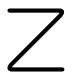
\includegraphics[keepaspectratio]{images/part001_bd86b8f3.jpg}}

换言之，当 I 无界时，若以 \(\mathcal{I}\) 表示由 I 上的规则函数 \(\mathbf{f}\)（取值于 E 且在 I 上有一个积分）所构成的向量空间，则映射 \(\mathbf{f} \mapsto \int_{\mathrm{I}} \mathbf{f}(t) dt\) 在 \(\mathcal{I}\) 赋以 I 上一致收敛的拓扑之后不是连续的（参见 II, p.~53, 推论 2）。

我们将在下列假设之下寻求保证命题 1 成立的充分条件：

\(1^{\circ}\) I 是 \(\mathbf{R}\) 中的任意区间，函数 \(\mathbf{f}_{\alpha}\) 在 I 上是规则的，并且在 I 上有一个积分；

\(2^{\circ}\) 族 \((\mathbf{f}_{\alpha})\) 在含于 I 的每个紧区间上一致收敛于 \(\mathbf{f}\)（关于滤子 \(\mathfrak{F}\)）。

以 \(\mathfrak{K}(\mathrm{I})\) 表示含于 I 的紧区间所成的有向集（II, p.~64），II, p.~68 的公式 (1) 的左端可以写成 \(\lim_{\mathfrak{F}}\left(\lim_{\mathrm{J}\in \mathfrak{K}(\mathrm{I})}\int_{\mathrm{J}}\mathbf{f}_{\alpha}(t)dt\right)\)；
另一方面，考虑到命题 1（II, p.~68）以及族 \((\mathbf{f}_{\alpha})\) 在每个紧区间 \(J \subset I\) 上一致收敛这一事实，(1)（II, p.~68）的右端可以写成 \(\lim_{\mathrm{J} \in \mathfrak{K}(\mathrm{I})} \left( \lim_{\mathfrak{F}} \int_{\mathrm{J}} \mathbf{f}_{\alpha}(t) dt \right)\)。由此看出，只要
对映射 (J, \(\alpha\) ) \(\mapsto \int_{J} f_{\alpha}(t) dt\) 关于滤子 F 以及关于有向集 K(I) 的截口滤子 \(\Phi\) 可以交换极限，II, p.~19 的命题 1 就可以推广。现在，我们知道使这一交换合法的一个充分条件，即映射 (J, \(\alpha\) ) \(\mapsto \int_{J} f_{\alpha}(t) dt\) 关于乘积滤子 \(\Phi \times F\) 的极限存在（Gen.~Top., I, p.~81, 定理 1 的推论）。我们将把这个条件变换为一个等价的、更便于使用的条件。

首先，由于 E 是完备的，为使 \((\mathbf{J}, \alpha) \mapsto \int_{\mathbf{J}} \mathbf{f}_{\alpha}(t) dt\) 关于 \(\Phi \times F\) 有极限，必须且只需：对每个 \(\varepsilon > 0\)，存在一个紧区间 \(J_{0} \subset I\) 和一个集 \(M \in F\)，使得对 M 中任意的元素 \(\alpha\)、\(\beta\) 以及任意的含于 I 的紧区间 \(J \supset J_{0}\)，有

\[
\left\| \int_ {J _ {0}} \mathbf {f} _ {\alpha} (t) d t - \int_ {J} \mathbf {f} _ {\beta} (t) d t \right\| \leqslant \varepsilon .\tag{4}
\]

另一方面我们将证明，这个条件本身等价于下列条件：对每个 \(\varepsilon > 0\)，存在一个紧区间 \(J_0 \subset I\) 和一个集 \(M \in \mathfrak{F}\)，使得对任意的 \(\alpha\)（属于 \(M\)）以及任意的紧区间 \(J \supset J_0\)（含于 \(I\)），有

\[
\left\| \int_ {J _ {0}} \mathbf {f} _ {\alpha} (t) d t - \int_ {J} \mathbf {f} _ {\alpha} (t) d t \right\| \leqslant \varepsilon .\tag{5}
\]

的确，明显可见后一条件是必要的；反之，若它满足，则（由 \((\mathbf{f}_{\alpha})\) 在每个紧区间上的一致收敛性）存在一个集 \(N \in F\)，使得对 N 中任意的 \(\alpha\)、\(\beta\)，有

\[
\left\| \int_ {\mathrm{J} _ {0}} \mathbf {f} _ {\alpha} (t) d t - \int_ {\mathrm{J} _ {0}} \mathbf {f} _ {\beta} (t) d t \right\| \leqslant \varepsilon ;\tag{6}
\]

因而有 \(\left\|\int_{J_{0}}\mathbf{f}_{\alpha}(t)dt-\int_{J}\mathbf{f}_{\beta}(t)dt\right\|\leqslant2\varepsilon\)（对任意的 \(\alpha\) 与 \(\beta\)（属于 \(M\cap N\in\mathfrak{F}\)）以及任意的紧区间 \(J\supset J_{0}\)）。

最后，II, p.~65 的引理使我们能把后一条件写成下列等价形式：对每个 \(\varepsilon > 0\)，存在一个紧区间 \(\mathbf{J}_0 \subset \mathbf{I}\) 和一个集 \(\mathbf{M} \in \mathfrak{F}\)（依赖于 \(\varepsilon\)），使得对每个紧区间 \(\mathbf{K} \subset \mathbf{I}\)（与 \(\mathbf{J}_0\) 无公共内点）以及每个 \(\alpha \in \mathbf{M}\)，有 \(\left\| \int_{\mathbf{K}} \mathbf{f}_{\alpha}(t) dt \right\| \leqslant \varepsilon\)。

最常用的，是一个更强的条件，它是在上述结论中假设集 M 不依赖于 \(\varepsilon\) 而得到的：

定义 1. 我们说积分 \(\int_{\mathrm{I}} \mathbf{f}_{\alpha}(t) dt\) 对 \(\alpha \in \mathrm{A}\) 一致收敛（或在 \(\mathrm{A}\) 上一致收敛），如果对每个 \(\varepsilon > 0\)，存在一个紧区间 \(\mathrm{J}_0 \subset J\)，使得对每个紧区间 \(\mathrm{K} \subset \mathrm{I}\)（与 \(\mathrm{J}_0\) 无公共内点）以及每个 \(\alpha \in \mathrm{A}\)，有

\[
\left\| \int_ {K} \mathbf {f} _ {\alpha} (t) d t \right\| \leqslant \varepsilon .\tag{7}
\]

这个定义等价于说：映射族 \(\alpha\mapsto\int_{J}\mathbf{f}_{\alpha}(t)dt\) 在 A 上一致收敛（收敛于映射 \(\alpha\mapsto\int_{I}\mathbf{f}_{\alpha}(t)dt\)），即关于滤子 \(\Phi\)（\(\Re(I)\) 的截口滤子）而言；诸积分 \(\int_{I}\mathbf{f}_{\alpha}(t)dt\) 中的每一个更是收敛的（反之不真）；此外，由我们刚才所见（或由 Gen.~Top., X, p.~281, 推论 2）：

命题 3. 设 \((\mathbf{f}_{\alpha})\) 是区间 I 上的一个规则函数族，满足：\(1^{\circ}\) 关于滤子 \(\mathfrak{F}\)，族 \((\mathbf{f}_{\alpha})\) 在含于 I 的每个紧区间上一致收敛于一个函数 \(\mathbf{f}\)（在 I 上是规则的）；\(2^{\circ}\) 积分 \(\int_{I} \mathbf{f}_{\alpha}(t) dt\) 对每个 \(\alpha \in A\) 一致收敛。在这些假设之下，积分 \(\int_{I} \mathbf{f}(t) dt\) 收敛，且有

\[
\lim _ {\mathfrak {F}} \int_ {\mathrm{I}} \mathbf {f} _ {\alpha} (t) d t = \int_ {\mathrm{I}} \mathbf {f} (t) d t.\tag{8}
\]

例如当 I 是有界区间、\(\mathbf{f}_{\alpha}\) 在 I 上一致有界且在含于 I 的每个紧区间上一致收敛于 \(\mathbf{f}\) 时，命题 3 的假设满足；事实上，若 \(\| \mathbf{f}_{\alpha}(x)\| \leqslant h\) 对一切 \(x\in \mathrm{I}\) 与一切 \(\alpha\) 成立，且 \(\mathrm{J}_0\) 使得 I 与 \(\mathrm{J}_0\) 的长度之差 \(\leqslant \varepsilon /h\)，则对每个区间 \(\mathrm{K}\subset \mathrm{I}\)（与 \(\mathrm{J}_0\) 无公共内点），条件 (7) 满足。

与 II, p.~68 的命题 1 一样，命题 3 的两个推论在应用中很重要：

推论 1. 设 \((\mathbf{f}_{n})\) 是任意区间 I 上的一个规则函数序列，在含于 I 的每个紧区间上一致收敛于函数 f；若积分 \(\int_{I} \mathbf{f}_{n}(t) dt\) 一致收敛，则积分 \(\int_{I} \mathbf{f}(t) dt\) 收敛，且

\[
\lim _ {n \to \infty} \int_ {\mathrm{I}} \mathbf {f} _ {n} (t) d t = \int_ {\mathrm{I}} \mathbf {f} (t) d t.\tag{9}
\]

注记。这个推论中所加的假设对公式 (9) 的成立是充分的，但不是必要的；以后我们将在推广积分概念的同时推广这个公式（见 INT, IV），并得到弱得多的条件。

推论 2. 设 A 是拓扑空间 F 的一个子集，f 是 I × A 到 R 上的完备赋范空间 E 中的一个映射，使得对每个 \(\alpha \in A\)，函数 \(x \mapsto \mathbf{f}(x, \alpha)\) 在 I 上是规则的。若一方面，函数 \(x \mapsto \mathbf{f}(x, \alpha)\) 在含于 I 的每个紧区间上一致收敛于函数 \(x \mapsto \mathbf{f}(x)\)（当 \(\alpha\) 趋于 \(\alpha_{0} \in \overline{A}\) 而保持属于 A 时）；若另一方面，积分 \(\int_{I} \mathbf{f}(x, \alpha) dx\) 在 A 上一致收敛，则积分 \(\int_{I} \mathbf{f}(x) dx\) 收敛，且有

\[
\lim _ {\alpha \rightarrow \alpha_ {0}, \alpha \in A} \int_ {I} \mathbf {f} (x, \alpha) d x = \int_ {I} \mathbf {f} (x) d x.\tag{10}
\]

特别地：

命题 4（“反常积分对参数的连续性”）。设 F 是紧空间，I 是 R 中的任意区间，f 是 I × F 到 R 上的完备赋范空间 E 中的连续映射；若积分 \(\mathbf{h}(\alpha) = \int_{\mathrm{I}} \mathbf{f}(x, \alpha) dx\) 在 F 上一致收敛，则它是 \(\alpha\) 在 F 上的连续函数。

由于 II, p.~69 的命题 2，本命题也可由连续函数的一致极限的连续性（Gen.~Top., X, p.~282, 定理 2）得出。

\subsection{正规收敛积分}

设 \((\mathbf{f}_{\alpha})_{\alpha\in\mathrm{A}}\) 是任意区间 \(I\subset R\) 上的一个规则函数族，取值于 R 上的完备赋范空间 E 中。假设存在 I 上的一个有限实规则函数 g，使得对每个 \(x\in I\) 与每个 \(\alpha\in A\)，\(\|f_{\alpha}(x)\|\leqslant g(x)\)，并且积分 \(\int_{I}g(t)dt\) 收敛。在这些条件之下，积分 \(\int_{I}\mathbf{f}_{\alpha}(t)dt\) 在 A 上绝对且一致收敛；事实上，对含于 I 的每个紧区间 K，

\[
\left\| \int_ {K} \mathbf {f} _ {\alpha} (t) d t \right\| \leqslant \int_ {K} g (t) d t
\]

而积分 \(\int_{I} g(t) dt\) 的收敛性蕴含：对每个 \(\varepsilon > 0\)，存在一个紧区间 \(J \subset I\)，使得对每个与 J 不相交的紧区间 \(K \subset I\)，有 \(\int_{K} g(t) dt \leqslant \varepsilon\)。当存在一个具有上述性质的实函数 g 时，我们就说积分 \(\int_{I} f_{\alpha}(t) dt\) 在 A 上正规收敛（参见 Gen.~Top., X, p.~296）。

一个积分可以在 A 上一致收敛而非正规收敛。*实函数序列 \((f_n)\) 由下列条件定义：\(f_n(x) = 1 / x\)（当 \(n \leqslant x \leqslant n + 1\)），\(f_n(x) = 0\)（当 \(x\) 在 \(\mathbf{I} = [\mathbf{0}, +\infty[\) 中取其他值），对它就出现这种情形。立即可以看出，积分 \(\int_{1}^{\infty} f_n(t) dt\) 一致收敛，但非正规收敛，因为关系式 \(g(x) \geqslant f_n(x)\)（对每个 \(x \in \mathbf{I}\) 与所有 \(n\)）蕴含 \(g(x) \geqslant 1 / x\)，从而 \(g\) 在 \(\mathbf{I}\) 上的积分不收敛。*

特别地，考虑一个级数，其通项 \(u_{n}\) 是区间 I 上的规则函数，并假设以 \(\|u_{n}(x)\|\)（它是 I 上的规则函数）为通项的级数在含于 I 的每个紧区间上一致收敛，且以 \(\int_{I}\|\mathbf{u}_{n}(t)\|dt\) 为通项的级数收敛；于是（II, p.~66, 命题 2）（规则的）函数 \(g(x)\)——即以 \(\|u_{n}(x)\|\) 为通项的级数之和——使得积分 \(\int_{I}g(t)dt\) 收敛。若令 \(f_{n}=\sum_{p=1}^{n}u_{p}\)，则积分 \(\int_{I}f_{n}(t)dt\) 正规收敛，因为有

\[
\left\| \mathbf {f} _ {n} (x) \right\| \leqslant \sum_ {p = 1} ^ {n} \left\| \mathbf {u} _ {p} (x) \right\| \leqslant g (x)
\]

对一切 \(x \in \mathrm{I}\) 与一切 \(n\) 成立；因此，和 \(\mathbf{f}\)——即以 \(\mathbf{u}_n\) 为通项的级数之和——是 \(\mathrm{I}\) 上的规则函数，且积分 \(\int_{\mathrm{I}} \mathbf{f}(t) dt\) 收敛，并有

\[
\int_ {\mathrm{I}} \mathbf {f} (t) d t = \sum_ {n = 1} ^ {\infty} \int_ {\mathrm{I}} \mathbf {u} _ {n} (t) d t\tag{11}
\]

（“非紧区间上级数的逐项积分”）。

\subsection{紧区间上积分对参数的导数}

设 A 是域 R（相应地，域 C）中一点 \(\alpha_{0}\) 的紧邻域，I = {[}a, b{]} 是 R 中的紧区间，f 是 I × A 到 R（相应地，C）上的完备赋范空间 E 中的连续映射。我们已经看到（II, p.~69, 命题 2），在这些条件之下 \(\mathbf{g}(\alpha) = \int_{a}^{b} \mathbf{f}(t, \alpha) dt\) 是 A 上的连续函数。我们来寻求使 g 在点 \(\alpha_{0}\) 处有导数的充分条件。对 \(\alpha \neq \alpha_{0}\)，有

\[
\frac {\mathbf {g} (\alpha) - \mathbf {g} (\alpha_ {0})}{\alpha - \alpha_ {0}} = \int_ {a} ^ {b} \frac {\mathbf {f} (t , \alpha) - \mathbf {f} (t , \alpha_ {0})}{\alpha - \alpha_ {0}} d t
\]

因而（II, p.~69, 推论 2），若函数 \(x \mapsto \frac{\mathbf{f}(x, \alpha) - \mathbf{f}(x, \alpha_0)}{\alpha - \alpha_0}\) 在 I 上一致收敛于一个（必然连续的）函数 \(x \mapsto \mathbf{h}(x)\)（当 \(\alpha\) 趋于 \(\alpha_0\) 而保持 \(\neq \alpha_0\) 时），则 \(\mathbf{g}\) 有一个等于 \(\int_{a}^{b} \mathbf{h}(t) dt\) 的导数（在点 \(\alpha_0\) 处）；此外，对每个 \(x \in I\)，\(\frac{\mathbf{f}(x, \alpha) - \mathbf{f}(x, \alpha_0)}{\alpha - \alpha_0}\) 趋于 \(\mathbf{h}(x)\)，故 \(\mathbf{h}(x)\) 是在点 \(\alpha_0\) 处映射 \(\alpha \mapsto \mathbf{f}(x, \alpha)\) 的导数；我们把这个导数（称为 \(\mathbf{f}\) 关于 \(\alpha\) 的偏导数）记作 \(\mathbf{f}_{\alpha}'(x, \alpha_0)\)；我们所做的假设蕴含

\[
\mathbf {g} ^ {\prime} (\alpha_ {0}) = \int_ {a} ^ {b} \mathbf {f} _ {\alpha} ^ {\prime} (t, \alpha_ {0}) d t.\tag{12}
\]

下面的命题给出使公式 (12) 成立的一个非常简单的充分条件：

命题 5. 假设偏导数 \(\mathbf{f}_{\alpha}^{\prime}(x,\alpha)\) 对所有 \(x\in \mathrm{I}\) 与所有 \(\alpha\)（属于 \(\mathbf{V}\)，即 \(\alpha_0\) 的一个开邻域）存在，并且对所有 \(\alpha \in \mathbf{V}\)，映射 \(x\mapsto \mathbf{f}_{\alpha}^{\prime}(x,\alpha)\) 在 \(\mathrm{I}\) 上是规则的。在这些条件之下，若 \(x\mapsto \mathbf{f}_{\alpha}^{\prime}(x,\alpha)\) 在 \(\mathrm{I}\) 上一致收敛于 \(x\mapsto \mathbf{f}_{\alpha}^{\prime}(x,\alpha_0)\)（当 \(\alpha\) 趋于 \(\alpha_0\) 时），则函数 \(\mathbf{g}(\alpha) = \int_{a}^{b}\mathbf{f}(t,\alpha)dt\) 有一个由公式 (12) 给出的导数（在点 \(\alpha_0\) 处）。

事实上，对每个 \(\varepsilon > 0\)，由假设存在一个 \(r > 0\)，使得 \(|\alpha - \alpha_0| \leqslant r\) 蕴含 \(\left\| \mathbf{f}_{\alpha}'(x, \alpha) - \mathbf{f}_{\alpha}'(x, \alpha_0) \right\| \leqslant \varepsilon\)（对任何 \(x \in I\)）。由 I, p.~17 的命题 3 与命题 5，对 \(|\alpha - \alpha_0| \leqslant r\)（\(\alpha \neq \alpha_0\)）与所有 \(x \in I\)，有

\[
\left| \left| \frac {\mathbf {f} (x , \alpha) - \mathbf {f} (x , \alpha_ {0})}{\alpha - \alpha_ {0}} - \mathbf {f} _ {\alpha} ^ {\prime} (x, \alpha_ {0}) \right| \right| \leqslant \varepsilon
\]

这就证明了 \(\frac{\mathbf{f}(x,\alpha)-\mathbf{f}(x,\alpha_{0})}{\alpha-\alpha_{0}}\) 一致收敛于 \(\mathbf{f}_{\alpha}^{\prime}(x,\alpha_{0})\)（在 I 上，当 \(\alpha\) 趋于 \(\alpha_{0}\) 且保持 \(\neq\alpha_{0}\) 时），从而建立了公式 (12)。

推论。若偏导数 \(\mathbf{f}_{\alpha}^{\prime}(x,\alpha)\) 在 I × V 上存在且是 \((x,\alpha)\) 在这个集合上的连续函数，则函数 g 在点 \(\alpha_{0}\) 处有一个由公式 (12) 给出的导数。

事实上，若 W 是含于 V 的 \(\alpha_{0}\) 的紧邻域，则映射 \((x,\alpha)\mapsto\mathbf{f}_{\alpha}^{\prime}(x,\alpha)\) 在紧集 I × W 上一致连续，故 \(\mathbf{f}_{\alpha}^{\prime}(x,\alpha)\) 一致收敛于 \(\mathbf{f}_{\alpha}^{\prime}(x,\alpha_{0})\)（在 I 上，当 \(\alpha\) 趋于 \(\alpha_{0}\) 时）。

由命题 5 可以推出一个更一般的命题，它使我们在被积函数 f 以及积分限都依赖于一个参数 \(\alpha\) 时也能求出积分的导数：

命题 6. 在命题 5 的假设满足之下，设 \(a(\alpha)\)、\(b(\alpha)\) 是定义在 V 上、取值于 I 中的两个函数；若导数 \(a'(\alpha_0)\)、\(b'(\alpha_0)\) 存在且有限，则函数 \(\mathbf{g}(\alpha) = \int_{a(\alpha)}^{b(\alpha)} \mathbf{f}(t, \alpha) dt\) 在 \(\alpha_0\) 处有一个由下式给出的导数

\[
\mathbf {g} ^ {\prime} (\alpha_ {0}) = \int_ {a (\alpha_ {0})} ^ {b (\alpha_ {0})} \mathbf {f} _ {\alpha} ^ {\prime} (t, \alpha_ {0}) d t + b ^ {\prime} (\alpha_ {0}) \mathbf {f} (b (\alpha_ {0}), \alpha_ {0}) - a ^ {\prime} (\alpha_ {0}) \mathbf {f} (a (\alpha_ {0}), \alpha_ {0}).\tag{13}
\]

事实上，对所有 \(\alpha \in \mathbf{V}\)（异于 \(\alpha_0\)），可以写出

\[
\begin{array}{c} \frac {\mathbf {g} (\alpha) - \mathbf {g} (\alpha_ {0})}{\alpha - \alpha_ {0}} = \int_ {a (\alpha_ {0})} ^ {b (\alpha_ {0})} \frac {\mathbf {f} (t , \alpha) - \mathbf {f} (t , \alpha_ {0})}{\alpha - \alpha_ {0}} d t + \frac {1}{\alpha - \alpha_ {0}} \int_ {b (\alpha_ {0})} ^ {b (\alpha)} \mathbf {f} (t, \alpha) d t \\ - \frac {1}{\alpha - \alpha_ {0}} \int_ {a (\alpha_ {0})} ^ {a (\alpha)} \mathbf {f} (t, \alpha) d t. \end{array}
\]

由 II, p.~74 的命题 5，右端的第一个积分趋于 \(\int_{a(\alpha_0)}^{b(\alpha_0)} \mathbf{f}'_\alpha(t, \alpha_0) dt\)（当 \(\alpha\) 趋于 \(\alpha_0\) 时）。在第二个积分中，我们把 \(\mathbf{f}(t, \alpha)\) 换成 \(\mathbf{f}(b(\alpha_0), \alpha_0)\)，并证明其差趋于 0。令 \(\mathbf{M} = \operatorname{Max}\big( \| \mathbf{f}(b(\alpha_0), \alpha_0) \|, |b'(\alpha_0)| + 1 \big)\)；由于函数 \(b(\alpha)\) 在点 \(\alpha_0\) 连续，函数 \(\mathbf{f}\) 在点 \((b(\alpha_0), \alpha_0)\) 连续，故对每个 \(\varepsilon\)（满足 \(0 < \varepsilon < 1\)）存在一个 \(r > 0\)，使得关系 \(|\alpha - \alpha_0| \leqslant r\) 蕴含 \(\| \mathbf{f}(t, \alpha) - \mathbf{f}(b(\alpha_0), \alpha_0) \| \leqslant \varepsilon\)（对所有 \(t\)，它属于以 \(b(\alpha_0)\) 与 \(b(\alpha)\) 为端点的区间）；于是还可以假设关系 \(|\alpha - \alpha_0| \leqslant r\) 蕴含 \(\left| \frac{b(\alpha) - b(\alpha_0)}{\alpha - \alpha_0} - b'(\alpha_0) \right| \leqslant \varepsilon\)。

于是，由中值公式（II, p.~62, 公式 (17)）有

\[
\left\| \frac {1}{\alpha - \alpha_ {0}} \int_ {b (\alpha_ {0})} ^ {b (\alpha)} \mathbf {f} (t, \alpha) d t - \frac {b (\alpha) - b (\alpha_ {0})}{\alpha - \alpha_ {0}} \mathbf {f} (b (\alpha_ {0}), \alpha_ {0}) \right\| \leqslant \left| \frac {b (\alpha) - b (\alpha_ {0})}{\alpha - \alpha_ {0}} \right| \varepsilon
\]

从而

\[
\left\| \frac {1}{\alpha - \alpha_ {0}} \int_ {b (\alpha_ {0})} ^ {b (\alpha)} \mathbf {f} (t, \alpha) d t - b ^ {\prime} (\alpha_ {0}) \mathbf {f} (b (\alpha_ {0}), \alpha_ {0}) \right\| \leqslant 2 \mathrm{M} \varepsilon
\]

这表明 \(\frac{1}{\alpha - \alpha_0} \int_{b(\alpha_0)}^{b(\alpha)} \mathbf{f}(t, \alpha) dt\) 趋于 \(b'(\alpha_0)\mathbf{f}(b(\alpha_0), \alpha_0)\)。同理可证 \(\frac{1}{\alpha - \alpha_0} \int_{a(\alpha_0)}^{a(\alpha)} \mathbf{f}(t, \alpha) dt\) 趋于 \(a'(\alpha_0)\mathbf{f}(a(\alpha_0), \alpha_0)\)。

\subsection{非紧区间上积分对参数的导数}

设集 V 与 II, p.~74 的命题 5 中的含义相同，现在假设 I 是 R 中的任意区间，f 是 I × V 到 E 中的连续映射；若积分 \(\mathbf{g}(\alpha) = \int_{\mathrm{I}} \mathbf{f}(t, \alpha) dt\) 对所有 \(\alpha \in V\) 存在且是 \(\alpha\) 的连续函数，则函数 g 未必有一个等于 \(\int_{\mathrm{I}} \mathbf{f}'_{\alpha}(t, \alpha_0) dt\) 的导数（在点 \(\alpha_0\) 处），即使 \(\mathbf{f}'_{\alpha}(x, \alpha)\)

在含于 I 的每个紧区间上一致收敛于 \(\mathbf{f}_{\alpha}^{\prime}(x,\alpha_{0})\)，且积分 \(\int_{\mathrm{I}}\mathbf{f}_{\alpha}^{\prime}(t,\alpha)dt\) 对所有 \(\alpha \in \mathrm{V}\) 存在（参见 II, p.~87, 习题 3）。

下面的命题给出了使公式 (12)（II, p.~74）仍然成立的一个充分条件：

命题 7. 设 I 是 \(\mathbf{R}\) 中的任意区间，\(\mathbf{f}\) 是 \(\mathrm{I} \times \mathrm{V}\) 上的连续函数。假设：

\(1^{\circ}\) 偏导数 \(\mathbf{f}_{\alpha}^{\prime}(x,\alpha)\) 对所有 \(x\in \mathrm{I}\) 与所有 \(\alpha \in \mathrm{V}\) 存在，且对所有 \(\alpha \in \mathrm{V}\)，映射 \(x\mapsto \mathbf{f}_{\alpha}^{\prime}(x,\alpha)\) 在 \(\mathrm{I}\) 上是规则的；

\(2^{\circ}\) 对所有 \(\alpha \in \mathrm{V}\)，\(\mathbf{f}_{\alpha}^{\prime}(x,\beta)\) 一致收敛于 \(\mathbf{f}_{\alpha}^{\prime}(x,\alpha)\)（在含于 I 的每个紧区间上，当 \(\beta\) 趋于 \(\alpha\) 时）；

\(3^{\circ}\) 积分 \(\int_{\mathrm{I}}\mathbf{f}_{\alpha}^{\prime}(t,\alpha)dt\) 在 \(\mathrm{V}\) 上一致收敛；

\(4^{\circ}\) 积分 \(\int_{\mathrm{I}}\mathbf{f}(t,\alpha_0)dt\) 收敛。

在这些条件之下，积分 \(\mathbf{g}(\alpha)=\int_{\mathrm{I}}\mathbf{f}(t,\alpha)dt\) 在 V 上一致收敛，且函数 g 在 V 的每一点处有一个由下式给出的导数

\[
\mathbf {g} ^ {\prime} (\alpha) = \int_ {\mathrm{I}} \mathbf {f} _ {\alpha} ^ {\prime} (t, \alpha) d t.\tag{14}
\]

\(\int_{\mathrm{I}} \mathbf{f}_{\alpha}'(t, \alpha) dt\) 在 V 上的一致收敛意味着：函数 \(\alpha \mapsto \int_{\mathrm{J}} \mathbf{f}_{\alpha}'(t, \alpha) dt\) 在 V 上关于滤子 \(\Phi\)——即有向集 \(\Re(\mathrm{I})\)（由含于 I 的紧区间 J 组成）的截口滤子——一致收敛。令 \(\mathbf{u}_{\mathrm{J}}(\alpha) = \int_{\mathrm{J}} \mathbf{f}(t, \alpha) dt\)；这些假设表明，一方面 \(\mathbf{u}_{\mathrm{J}}(\alpha_0)\) 关于 \(\Phi\) 有一个极限，另一方面，由 II, p.~74 的命题 5，有 \(\mathbf{u}_{\mathrm{J}}'(\alpha) = \int_{\mathrm{J}} \mathbf{f}_{\alpha}'(t, \alpha) dt\)（对一切 \(\alpha \in \mathrm{V}\)）。因此我们可以把 II, p.~52 的定理 1 应用于函数 \(\mathbf{u}_{\mathrm{J}}\)，这里指标集的角色由 \(\Re(\mathrm{I})\) 扮演，而这个集合上的滤子的角色由滤子 \(\Phi\) 扮演；命题随之立得。

注记。1) 命题 7 的条件 \(1^{\circ}\) 与 \(2^{\circ}\) 更是满足的，当 \(\mathbf{f}_{\alpha}^{\prime}(x,\alpha)\) 是 \((x,\alpha)\) 在 \(\mathrm{I} \times \mathrm{V}\) 上的连续函数时。

\begin{enumerate}
\def\labelenumi{\arabic{enumi})}
\setcounter{enumi}{1}
\tightlist
\item
  在积分 \(\int_{a(\alpha)}^{b(\alpha)}\mathbf{f}(t,\alpha)dt\) 中，当区间的端点是参数的有限函数时，把这个积分作为 \(\alpha\) 的函数来研究可以化为对 {[}0, 1{]} 上积分的研究；事实上，通过变量替换 \(t = a(\alpha)(1 - u) + b(\alpha)u\)，有
\end{enumerate}

\[
\int_ {a (\alpha)} ^ {b (\alpha)} \mathbf {f} (t, \alpha) d t = \int_ {0} ^ {1} \mathbf {f} (a (\alpha) (1 - u) + b (\alpha) u, \alpha) (b (\alpha) - a (\alpha)) d u.
\]

\subsection{积分次序的交换}

设 \(I = [a, b]\) 与 \(A = [c, d]\) 是 \(R\) 中的两个紧区间；设 \(f\) 是 \(I \times A\) 上的连续函数，取值于完备赋范空间 \(E\)（定义在 \(R\) 上）中；由 II, p.~69 的命题 2，\(\int_{a}^{b} f(x, \alpha) dx\) 是 \(\alpha\) 在 \(A\) 上的连续函数；为简单起见，它的积分 \(\int_{c}^{d} \left( \int_{a}^{b} f(x, \alpha) dx \right) d\alpha\) 也记作 \(\int_{c}^{d} d\alpha \int_{a}^{b} f(x, \alpha) dx\)。

命题 8. 若 \(\mathbf{f}\) 在 \(\mathrm{I} \times \mathrm{A}\) 上连续，则有

\[
\int_ {c} ^ {d} d \alpha \int_ {a} ^ {b} \mathbf {f} (x, \alpha) d x = \int_ {a} ^ {b} d x \int_ {c} ^ {d} \mathbf {f} (x, \alpha) d \alpha\tag{15}
\]

（“交换积分次序的公式”）。

我们将证明，对所有 \(y \in A\)，有

\[
\int_ {c} ^ {y} d \alpha \int_ {a} ^ {b} \mathbf {f} (x, \alpha) d x = \int_ {a} ^ {b} d x \int_ {c} ^ {y} \mathbf {f} (x, \alpha) d \alpha .\tag{16}
\]

由于 (16) 的两端都是 \(y\) 的函数，且在 \(y = c\) 时相等，故只需证明它们在 \(]c\) , \(d[\) 上可微且其导数在这个区间的每一点处相等。若令 \(\mathbf{g}(\alpha) = \int_{a}^{b} \mathbf{f}(x, \alpha) dx\) 与 \(\mathbf{h}(x, y) = \int_{c}^{y} \mathbf{f}(x, \alpha) dx\)，则关系式 (16) 可以写成

\[
\int_ {c} ^ {y} \mathbf {g} (\alpha) d \alpha = \int_ {a} ^ {b} \mathbf {h} (x, y) d x.
\]

而第一项对 \(y\) 的导数是 \(\mathbf{g}(y)\)，第二项的导数是 \(\int_{a}^{b} \mathbf{h}_{y}'(x, y) dx\)（由 II, p.74, 推论），因为 \(\mathbf{h}_{y}'(x, y) = \mathbf{f}(x, y)\) 在 \(I \times A\) 上连续；这样得到的两个表达式是相同的。

现在设 A = {[}c, d{]} 是 R 中的紧区间，I 是 R 中的任意区间；设 f 是 I × A 上的连续函数，取值于 E 中，使得积分 \(\mathbf{g}(\alpha) = \int_{\mathrm{I}} \mathbf{f}(t, \alpha) dt\) 对所有 \(\alpha \in A\) 收敛；即使 \(\mathbf{g}(\alpha)\) 在 A 上连续，也未必总能在积分 \(\int_{c}^{d} d\alpha \int_{I} \mathbf{f}(t, \alpha) dt\) 中交换积分次序，因为积分 \(\int_{I} dt \int_{c}^{d} \mathbf{f}(t, \alpha) d\alpha\) 可能不存在，或者可能与积分 \(\int_{c}^{d} d\alpha \int_{I} \mathbf{f}(t, \alpha) dt\) 不同（参见 II, p.~87, 习题 7）。然而有下列结果：

命题 9. 若函数 \(\mathbf{f}\) 在 \(\mathrm{I} \times \mathrm{A}\) 上连续，且积分 \(\int_{\mathrm{I}} \mathbf{f}(t, \alpha) dt\) 在 \(\mathrm{A}\) 上一致收敛，则积分 \(\int_{\mathrm{I}} dt \int_{c}^{d} \mathbf{f}(t, \alpha) d\alpha\) 收敛，且有

\[
\int_ {c} ^ {d} d \alpha \int_ {\mathrm{I}} \mathbf {f} (t, \alpha) d t = \int_ {\mathrm{I}} d t \int_ {c} ^ {d} \mathbf {f} (t, \alpha) d \alpha .\tag{17}
\]

对含于 I 的每个紧区间 J，令 \(\mathbf{u}_{\mathrm{J}}(\alpha) = \int_{\mathrm{J}} \mathbf{f}(t, \alpha) dt\)。这个假设蕴含：关于滤子 \(\Phi\)（有向集 \(\Re(\mathrm{I})\) 的截口滤子），连续函数 \(u_{J}\) 在 A 上一致收敛于 \(\int_{I} f(t, \alpha) dt\)；于是（II, p.~68, 命题 1），\(\int_{c}^{d} d\alpha \int_{J} f(t, \alpha) dt\) 有极限 \(\int_{c}^{d} d\alpha \int_{I} f(t, \alpha) dt\)（关于 \(\Phi\)）；但由命题 8（II, p.~77），有

\[
\int_ {c} ^ {d} d \alpha \int_ {\mathrm{J}} \mathbf {f} (t, \alpha) d t = \int_ {\mathrm{J}} d t \int_ {c} ^ {d} \mathbf {f} (t, \alpha) d \alpha .\tag{18}
\]

前面的结果于是表明积分 \(\int_{I} dt \int_{c}^{d} \mathbf{f}(t, \alpha) d\alpha\) 收敛，而且在关系式 (18) 中关于 \(\Phi\) 取极限，便得到 (17)。

\setcounter{exercisegroup}{0}
\refstepcounter{exercisegroup}
\section*{第 \S\arabic{exercisegroup} 节习题}
\phantomsection
\addcontentsline{toc}{section}{第 \protect\S\arabic{exercisegroup} 节习题}

\begin{enumerate}
\def\labelenumi{\arabic{enumi})}
\tightlist
\item
  设 \((f_{\alpha})\) 是一族实函数，定义在区间 \(\mathrm{I} \subset \mathbf{R}\) 上，其中每个函数在 \(\mathrm{I}\) 上有一个严格原函数，并且它们关于关系 \(\leqslant\) 构成一个有向集。设 \(f\) 是族 \((f_{\alpha})\) 的上包络；假设 \(f\) 在 \(\mathrm{I}\) 上有一个严格原函数。证明：若 \(g_{\alpha}\)（相应地，\(g\)）是 \(f_{\alpha}\)（相应地，\(f\)）的在点 \(x_0 \in \mathrm{I}\) 处为零的原函数，则 \(g\) 是族 \((g_{\alpha})\) 在交集 \(\mathrm{I} \cap [x_0, +\infty[\) 上的上包络，而是它在交集 \(\mathrm{I} \cap ] - \infty\) , \(x_0]\) 上的下包络。（限于这两个区间中的第一个，证明：若 \(u\) 是 \((g_{\alpha})\) 在 \(\mathrm{I} \cap [x_0, +\infty[\) 上的上包络，则 \(u(x + h) - u(x) \leqslant g(x + h) - g(x)\)（对 \(h > 0\)）成立；然后证明，对一切 \(\alpha\)，有 \(u(x + h) - u(x) \geqslant g_{\alpha}(x + h) - g_{\alpha}(x)\)，并由最后这个不等式断定 \(\liminf_{h \to 0} (u(x + h) - u(x))/h \geqslant f(x)\)；由此推出命题。）
\end{enumerate}

给出一个区间 I 上的递增连续函数序列 \((f_n)\) 的例子，这些函数一致有界，但其上包络在 I 上没有严格原函数。

\begin{enumerate}
\def\labelenumi{\arabic{enumi})}
\setcounter{enumi}{1}
\item
  证明：为使函数 \(\mathbf{f}\) 是区间 I 上的阶梯函数，必须且只需它只有有限个不连续点，并且在它连续的每个区间上取常值。
\item
  设 \(\mathbf{f}\) 是区间 \(I \subset \mathbf{R}\) 上的规则函数，取值于完备赋范空间 \(E\)（\(\mathbf{R}\) 上的）中；证明：对每个紧子集 \(H\)（含于 \(I\)），集合 \(\mathbf{f}(H)\) 在 \(E\) 中是相对紧的；给出一个 \(\mathbf{f}(H)\) 在 \(E\) 中不是闭集的例子。
\item
  给出一个连续实函数 \(f\)（在紧区间 \(\mathrm{I} \subset \mathbf{R}\) 上）的例子，使得复合函数 \(x \mapsto \operatorname{sgn}(f(x))\) 在 \(\mathrm{I}\) 上不是规则的（尽管 \(\operatorname{sgn}\) 在 \(\mathbf{R}\) 上是规则的）。
\item
  设 \(\mathbf{f}\) 是定义在紧区间 \(\mathrm{I} = [a, b] \subset \mathbf{R}\) 上、取值于完备赋范空间 \(\mathrm{E}\) 中的向量函数；我们说 \(\mathbf{f}\) 在 \(\mathrm{I}\) 上是有界变差的，如果存在一个数 \(m > 0\)，使得对每个有限的严格递增序列 \((x_i)_{0 \leqslant i \leqslant n}\)——由
\end{enumerate}

I 中满足 \(x_0 = a\) 与 \(x_n = b\) 的点组成——有 \(\sum_{i=0}^{n-1} \| \mathbf{f}(x_{i+1}) - \mathbf{f}(x_i) \| \leqslant m\)。

\begin{enumerate}
\def\labelenumi{\alph{enumi})}
\item
  证明 \(\mathbf{f}(\mathrm{I})\) 在 E 中相对紧（用反证法论证）。
\item
  证明 \(\mathbf{f}\) 在 I 上是规则的（证明当 \(x\) 趋于一点 \(x_0 \in \mathrm{I}\) 而保持 \(>x_0\) 时，函数 \(\mathbf{f}\) 不可能有两个不同的聚点，并利用 \(a\)））。
\end{enumerate}

\begin{enumerate}
\def\labelenumi{\arabic{enumi})}
\setcounter{enumi}{5}
\tightlist
\item
  为使函数 \(\mathbf{f}\)（取值于完备赋范空间 \(E\) 中、定义在开区间 \(I \subset R\) 上）在 \(I\) 的一个可数子集的余集的所有点处等于 \(I\) 上的一个规则函数，必须且只需它满足下列条件：对每个 \(x \in I\) 与每个 \(\varepsilon > 0\)，存在一个数 \(h > 0\) 和两个元素 \(a\)、\(b\)（\(E\) 的），使得 \(\| \mathbf{f}(y) - a \| \leqslant \varepsilon\) 对每个 \(y \in [x, x + h]\) 都成立（至多除去这个区间的可数无穷多个点），且 \(\| \mathbf{f}(z) - b \| \leqslant \varepsilon\) 对所有 \(z \in [x - h, x]\) 成立（至多除去这个区间的可数无穷多个点）。
\end{enumerate}

* 7) 证明：等于 \(\sin(1/x)\)（当 \(x \neq 0\)）而等于 0（当 \(x = 0\)）的函数在 \(\mathbf{R}\) 上有一个严格原函数（注意 \(x^2 \sin(1/x)\) 在每一点处有导数）。

由此推出：若 \(g(x,u,v)\) 是 u, v 的多项式，其系数是 x 在区间 I（包含 0）上的连续函数，则等于 \(g(x,\sin1/x,\cos1/x)\)（当 \(x\neq0\)）而等于一个适当的值 \(\alpha\)（待定）（当 x=0）的函数在 I 上有一个严格原函数；给出一个 \(\alpha\neq g(0,0,0)\) 的例子。

* 8) 证明：存在 \([-1, +1]\) 上的连续函数，在这个区间的每一点处有有限导数，这个导数等于 \(\sin\left(\frac{1}{\sin 1/x}\right)\)（在每一点 \(x\) 处，只要 x 异于 \(1/n\pi\)（\(n\) 为整数 \(\neq 0\)）且异于 0）。（在 \(x = 1/n\pi\) 的邻域内作变量替换 \(x = \frac{1}{n\pi + \operatorname{Arc} \sin u}\) 并利用习题 7；借助同样的变量替换证明，存在一个常数 \(a > 0\)（与 \(n\) 无关），使得

\[
\left| \int_ {2 / (2 n + 1) \pi} ^ {2 / (2 n - 1) \pi} \sin \left(\frac {1}{\sin \frac {1}{x}}\right) d x \right| \leqslant \frac {a}{n ^ {3}};
\]

并由此断定，若令

\[
g (x) = \lim _ {\varepsilon \rightarrow 0} \int_ {\varepsilon} ^ {x} \sin \left(\frac {1}{\sin \frac {1}{t}}\right) d t,
\]

则 g 在点 x = 0 处有一个等于 0 的导数。）*

\begin{enumerate}
\def\labelenumi{\arabic{enumi})}
\setcounter{enumi}{8}
\item
  设 \(\mathbf{f}\) 是紧区间 \(\mathrm{I} = [a, b]\) 上的规则函数。证明：对每个 \(\varepsilon > 0\)，存在一个连续函数 \(\mathbf{g}\)（在 \(\mathrm{I}\) 上），使得 \(\int_{a}^{b} \| \mathbf{f}(t) - \mathbf{g}(t) \| dt \leqslant \varepsilon\)（化为 \(\mathbf{f}\) 是阶梯函数的情形）。由此推出存在一个多项式 \(\mathbf{h}\)（系数在 E 中），使得 \(\int_{a}^{b} \| \mathbf{f}(t) - \mathbf{h}(t) \| dt \leqslant \varepsilon\)。
\item
  设 \(\mathbf{f}\) 是 \([a, b]\) 上的规则函数，取值于 E 中；设 \(\mathbf{g}\) 是 \([a, c]\)（\(c > b\)）上的规则函数，取值于 F 中；并设 \((\mathbf{x}, \mathbf{y}) \mapsto [\mathbf{x}, \mathbf{y}]\) 是 \(\mathrm{E} \times \mathrm{F}\) 到 G 中的连续双线性映射（E, F, G 是完备赋范空间）。证明
\end{enumerate}

\[
\lim _ {h \rightarrow 0, h > 0} \int_ {a} ^ {b} [ \mathbf {f} (t). \mathbf {g} (t + h) ] d t = \int_ {a} ^ {b} [ \mathbf {f} (t). \mathbf {g} (t) ] d t
\]

（化为 \(\mathbf{f}\) 是阶梯函数的情形）。

\begin{enumerate}
\def\labelenumi{\arabic{enumi})}
\setcounter{enumi}{10}
\tightlist
\item
  在与习题 10 相同的假设下，证明：对每个 \(\varepsilon > 0\)，存在一个数 \(\rho > 0\)，使得把 \([a, b]\) 分成区间 \([x_i, x_{i+1}]\)（长度 \(\leqslant \rho\)，\(0 \leqslant i \leqslant n-1\)）的每个分割，有
\end{enumerate}

\[
\left\| \int_ {a} ^ {b} [ \mathbf {f} (t). \mathbf {g} (t) ] d t - \sum_ {i = 0} ^ {n - 1} [ \mathbf {f} (u _ {i}). \mathbf {g} (v _ {i}) ] (x _ {i + 1} - x _ {i}) \right\| \leqslant \varepsilon
\]

对每个指标 i，不论点 \(u_{i}\)、\(v_{i}\)（取自 \([x_{i}, x_{i+1}]\)）如何选取（化为 f 与 g 都是阶梯函数的情形）。

¶ 12) 我们说实数序列 \((x_{n})\)（含于区间 \([0, 1]\)）在这个区间中是一致分布的，如果

\[
\lim _ {n \to \infty} \frac {\nu_ {n} (\alpha , \beta)}{n} = \beta - \alpha\tag{1}
\]

对每对数 \(\alpha\)、\(\beta\)（满足 \(0 \leqslant \alpha \leqslant \beta \leqslant 1\)）都成立，其中 \(\nu_{n}(\alpha, \beta)\) 表示指标 \(i\)（满足 \(1 \leqslant i \leqslant n\) 且 \(\alpha \leqslant x_{i} \leqslant \beta\)）的个数。

证明：若序列 \((x_{n})\) 一致分布且 \(\mathbf{f}\) 是 \([0, 1]\) 上的规则函数，则

\[
\lim _ {n \rightarrow \infty} \frac {1}{n} \sum_ {i = 1} ^ {n} \mathbf {f} (x _ {i}) = \int_ {0} ^ {1} \mathbf {f} (t) d t\tag{2}
\]

（化为 \(\mathbf{f}\) 是阶梯函数的情形）。逆命题。

证明：为使序列 \((x_{n})\) 一致分布，只需关系 (2) 对每个实函数 f（属于赋以一致收敛拓扑的 {[}0, 1{]} 上实连续函数空间中的一个稠密集）成立。

¶ 13) 设 \(f\) 是紧区间 \([a, b]\) 上的实规则函数。令

\[
r (n) = \frac {b - a}{n} \sum_ {k = 1} ^ {n} f \left(a + k \frac {b - a}{n}\right) - \int_ {a} ^ {b} f (t) d t.
\]

\begin{enumerate}
\def\labelenumi{\alph{enumi})}
\tightlist
\item
  证明：若 \(f\) 在 \([a, b]\) 上递增，则
\end{enumerate}

\[
0 \leqslant r (n) \leqslant \frac {b - a}{n} \Bigl (f (b) - f (a) \Bigr).
\]

\begin{enumerate}
\def\labelenumi{\alph{enumi})}
\setcounter{enumi}{1}
\tightlist
\item
  若 \(f\) 连续且在 \([a, b[\) 上有一个有界的规则右导数，证明有 \(\lim_{n\to \infty}nr(n) = \frac{b - a}{2} (f(b) - f(a))\)（令 \(x_{k} = a + k\frac{b - a}{n}\)），并注意有
\end{enumerate}

\[
r (n) = \sum_ {k = 0} ^ {n - 1} \int_ {x _ {k}} ^ {x _ {k + 1}} \left(f (x _ {k + 1}) - f (t)\right) d t,
\]

并应用 II, p.~57 的命题 5）。

\begin{enumerate}
\def\labelenumi{\alph{enumi})}
\setcounter{enumi}{2}
\tightlist
\item
  给出一个函数 \(f\) 的例子，它在 \([a, b]\) 上递增且连续，使得 \(nr(n)\) 不趋于 \(\frac{b - a}{2} (f(b) - f(a))\)（当 \(n\) 无限增大时） {[}取 \(f\) 为递增函数的递减序列 \((f_n)\) 的极限，这些递增函数的图象是折线，使得
\end{enumerate}

\[
f _ {n} \left(a + k \frac {b - a}{2 ^ {n}}\right) = f \left(a + k \frac {b - a}{2 ^ {n}}\right) \quad \text { for } \quad 0 \leqslant k \leqslant 2 ^ {n}
\]

且

\[
(b - a) \sum_ {k = 1} ^ {2 ^ {n}} f _ {n} \left(a + k \frac {b - a}{2 ^ {n}}\right) - 2 ^ {n} \int_ {a} ^ {b} f _ {n} (t) d t \geqslant \frac {3}{4} (b - a) \left(f _ {n} (b) - f _ {n} (a)\right) \Biggr ].
\]

\begin{enumerate}
\def\labelenumi{\arabic{enumi})}
\setcounter{enumi}{13}
\tightlist
\item
  设 \(\mathbf{f}\) 是一个向量函数，它是某个规则函数 \(\mathbf{f}'\)（在 \([a, b]\) 上）的原函数，且满足 \(\mathbf{f}(a) = \mathbf{f}(b) = 0\)。证明：若 \(\mathbf{M}\) 是 \(\| \mathbf{f}'(x)\|\) 在 \([a, b]\) 中使 \(\mathbf{f}'\) 连续的点所成之集上的上确界，则
\end{enumerate}

\[
\left\| \int_ {a} ^ {b} \mathbf {f} (t) d t \right\| \leqslant \mathrm{M} \frac {(b - a) ^ {2}}{4}.
\]

\begin{enumerate}
\def\labelenumi{\arabic{enumi})}
\setcounter{enumi}{14}
\tightlist
\item
  设 \(\mathbf{f}\) 是连续实函数，在区间 \([0, a]\) 上严格递增，且满足 \(f(0) = 0\)；设 \(g\) 是它的反函数，定义在 \([0, f(a)]\) 上且严格递增；证明
\end{enumerate}

\[
x y \leqslant \int_ {0} ^ {x} f (t) d t + \int_ {0} ^ {y} g (u) d u
\]

对 \(0 \leqslant x \leqslant a\) 与 \(0 \leqslant y \leqslant f(a)\) 成立，且仅当 \(y = f(x)\) 时取等号（把 \(xy - \int_{0}^{x} f(t) dt\) 作为 x 的函数研究其变差（y 固定））。由此推出：对 \(x \geqslant 0\)，\(y \geqslant 0\)，p \textgreater{} 1，\(p' = p/(p - 1)\)，有 \(xy \leqslant ax^{p} + by^{p'}\)（对 a \textgreater{} 0，b \textgreater{} 0 且 \((pa)^{p'}(p'b)^{p} \geqslant 1\)）。

\begin{enumerate}
\def\labelenumi{\arabic{enumi})}
\setcounter{enumi}{15}
\tightlist
\item
  设 \(\mathbf{f}\) 是 \(\mathrm{I} = [a, b] \subset \mathbf{R}\) 上的规则向量函数，\(\mathbf{u}\) 是 \(\mathbf{f}\) 在 \(\mathrm{I}\) 上的一个原函数，\(\mathrm{D}\) 是包含 \(\mathbf{u}(\mathrm{I})\) 的闭凸集。证明：若 \(g\) 是 \(\mathrm{I}\) 上的实单调函数，则
\end{enumerate}

\[
\int_ {a} ^ {b} \mathbf {f} (t) g (t) d t = (\mathbf {u} (b) - \mathbf {c}) g (b) + (\mathbf {c} - \mathbf {u} (a)) g (a)
\]

其中 \(\mathbf{c}\) 属于 D（化为 \(g\) 是单调阶梯函数的情形）。由此推出：若 \(f\) 是 I 上的实规则函数，则存在一个 \(c \in \mathrm{I}\)，使得

\[
\int_ {a} ^ {b} f (t) g (t) d t = g (a) \int_ {a} ^ {c} f (t) d t + g (b) \int_ {c} ^ {b} f (t) d t
\]

（“第二中值定理”）。

\begin{enumerate}
\def\labelenumi{\arabic{enumi})}
\setcounter{enumi}{16}
\tightlist
\item
  设 \(g\) 是实函数，有连续导数，且 \(\neq 0\)（在 \([a, x]\) 上）；若 \(f\) 是实函数，具有规则的 \((n + 1)^{th}\) 导数（在 \([a, x]\) 上），证明余项 \(r_n(x)\)——即 \(n\) 阶泰勒展开（\(f\) 在点 \(a\) 处的）中的余项——可以写成
\end{enumerate}

\[
r _ {n} (x) = (g (x) - g (a)) \frac {(x - \xi) ^ {n}}{n !} \frac {f ^ {(n + 1)} (\xi)}{g ^ {\prime} (\xi)}
\]

其中 \(a < \xi < x\)（利用 \(r_{n}(x)\) 的积分形式）。

\begin{enumerate}
\def\labelenumi{\arabic{enumi})}
\setcounter{enumi}{17}
\tightlist
\item
  设 \(f\) 是有限实函数，在开区间 \(I\) 上连续。为使 \(f\) 在 \(I\) 上是凸的，必须且只需对每个 \(x \in I\) 有
\end{enumerate}

\[
\operatorname * {l i m s u p} _ {h \to \infty} \left(\frac {1}{2 h} \int_ {x - h} ^ {x + h} f (t) d t - f (x)\right) \geqslant 0
\]

（按 I, p.~46 习题 9 的方式论证）。

\begin{enumerate}
\def\labelenumi{\arabic{enumi})}
\setcounter{enumi}{18}
\tightlist
\item
  设 \(f\) 是区间 \(I\) 上的凸函数，\(h\) 是一个数 \(> 0\)，\(I_h\) 是 \(I\) 与区间 \(I + h\)、\(I - h\) 的交；证明：若 \(I_h\) 非空，则函数
\end{enumerate}

\[
g _ {h} (x) = \frac {1}{2 h} \int_ {x - h} ^ {x + h} f (t) d t
\]

在 \(\mathrm{I}_h\) 上是凸的；若 \(h < k\)，则 \(g_h \leqslant g_k\)。证明：当 \(h\) 趋于 0 时，\(g_h\) 一致收敛于 \(f\)（在含于 \(\mathrm{I}\) 的内部的每个紧区间上）。

\begin{enumerate}
\def\labelenumi{\arabic{enumi})}
\setcounter{enumi}{19}
\tightlist
\item
  证明：当 \(n\) 无限增大时，多项式
\end{enumerate}

\[
f _ {n} (x) = \frac {\int_ {0} ^ {x} (1 - t ^ {2}) ^ {n} d t}{\int_ {0} ^ {1} (1 - t ^ {2}) ^ {n} d t}
\]

在每个区间 \([-1, -\varepsilon]\) 上一致收敛于 -1，而在每个区间 \([\varepsilon, +1]\) 上一致收敛于 +1，其中 \(\varepsilon > 0\)（注意 \(\int_{0}^{1}(1-t^{2})^{n}dt \geqslant \int_{0}^{1}(1-t)^{n}dt\)）。由此推出：多项式 \(g_{n}(x) = \int_{0}^{x} f_{n}(t)dt\) 一致收敛于 \(|x|\)（在 \([-1, +1]\) 上），这给出了魏尔斯特拉斯定理的一个新证明（Gen.~Top., X, p.~313, 命题 3）。

\begin{enumerate}
\def\labelenumi{\arabic{enumi})}
\setcounter{enumi}{20}
\tightlist
\item
  设 f 是区间 \([0, a]\) 上的实递增凸连续函数，且满足 \(f(0) = 0\)。若 \(a_{1} \geqslant a_{2} \geqslant \cdots \geqslant a_{n} \geqslant 0\) 是 \([0, a]\) 中点的一个有限递减序列，证明有
\end{enumerate}

\[
f \left(a _ {1}\right) - f \left(a _ {2}\right) + \dots + (- 1) ^ {n - 1} f \left(a _ {n}\right) \geqslant f \left(a _ {1} - a _ {2} + \dots + (- 1) ^ {n - 1} a _ {n}\right).
\]

（可以只限于 \(n = 2m\) 为偶数的情形；注意对 \(1 \leqslant j \leqslant m\) 有

\[
\int_ {\alpha} ^ {\beta} f ^ {\prime} (t) d t \leqslant \int_ {a _ {2 j}} ^ {a _ {2 j - 1}} f ^ {\prime} (t) d t
\]

其中 \(\alpha = a_{2j+1} - a_{2j+2} + \cdots + a_{2m-1} - a_{2m}\)，\(\beta = \alpha + (a_{2j-1} - a_{2j})\)。

\begin{enumerate}
\def\labelenumi{\arabic{enumi})}
\setcounter{enumi}{21}
\tightlist
\item
  设 f 是连续递增的实函数，且 \(\geqslant 0\)（在区间 {[}0, 1{]} 上）。
\end{enumerate}

\begin{enumerate}
\def\labelenumi{\alph{enumi})}
\item
  证明：存在一个凸函数 \(g \geqslant 0\)（在 {[}0,1{]} 上），使得 \(g \leqslant f\) 且 \(\int_0^1 g(t)dt \geqslant \frac{1}{2}\int_0^1 f(t)dt\)（参见 I, p.~48, 习题 23）。
\item
  证明：存在一个凸函数 \(h\)（在 {[}0, 1{]} 上），使得 \(h \geqslant f\)，并且
\end{enumerate}

\[
\int_ {0} ^ {1} h (t) d t \leqslant 2 \int_ {0} ^ {1} f (t) d t.
\]

（对每个 \(a\)（满足 \(0 < a \leqslant 1\)），令 \(f_a\) 是等于 \(f\)（当 \(0 \leqslant t \leqslant a\)）而等于 \(f(a)\)（当 \(a \leqslant t \leqslant 1\)）的函数；设 A 是使下列事实成立的 \(a \in [0,1]\) 所成的集：存在凸函数 \(h_a\)（在 \([0,1]\) 上），满足 \(h_a \geqslant f_a\) 且 \(\int_0^1 h_a(t)dt \leqslant 2\int_0^1 f_a(t)dt\)。证明上确界 \(b\)（A 的）仍属于 A，利用 I, p.~45 的习题 1。然后用反证法证明 \(f_{b} = f\)。为此，归结为证明下列结果：若 \(\varphi\) 在 \([0, 1]\) 上连续且递增、非常数、且满足 \(\varphi(0) = 0\)，则存在一点 \(c \in ]0, 1[\)，使得 \(\varphi(c) > 0\)，并且使得线性函数 \(\psi\)（满足 \(\psi(c) = \varphi(c)\) 及

\[
\psi (2 c - 1) = 0
\]

满足关系式 \(\psi(t) \geqslant \varphi(t)\)（对 \(\max(0, 2c - 1) \leqslant t \leqslant c\)）。

\begin{enumerate}
\def\labelenumi{\arabic{enumi})}
\setcounter{enumi}{22}
\tightlist
\item
  设 \(\mathbf{f}\) 是向量函数，在区间 \([a, b] \subset \mathbf{R}\) 上连续可微，取值于完备赋范空间中。
\end{enumerate}

\begin{enumerate}
\def\labelenumi{\alph{enumi})}
\tightlist
\item
  证明：对 \(a \leqslant t \leqslant b\)，有
\end{enumerate}

\[
\mathbf {f} (t) = \frac {1}{b - a} \int_ {a} ^ {b} \mathbf {f} (x) d x + \int_ {a} ^ {b} \frac {x - a}{b - a} \mathbf {f} ^ {\prime} (x) d x + \int_ {t} ^ {b} \frac {x - b}{b - a} \mathbf {f} ^ {\prime} (x) d x.
\]

\begin{enumerate}
\def\labelenumi{\alph{enumi})}
\setcounter{enumi}{1}
\tightlist
\item
  推出不等式
\end{enumerate}

\[
\| \mathbf {f} (t) \| \leqslant \frac {1}{b - a} \int_ {a} ^ {b} \| \mathbf {f} (x) \| d x + \int_ {a} ^ {b} \left\| \mathbf {f} ^ {\prime} (x) \right\| d x
\]

及

\[
\left\| \mathbf {f} \left(\frac {1}{2} (a + b)\right) \right\| \leqslant \frac {1}{b - a} \int_ {a} ^ {b} \| \mathbf {f} (x) \| d x + \frac {1}{2} \int_ {a} ^ {b} \left\| \mathbf {f} ^ {\prime} (x) \right\| d x.
\]

\setcounter{exercisegroup}{1}
\refstepcounter{exercisegroup}
\section*{第 \S\arabic{exercisegroup} 节习题}
\phantomsection
\addcontentsline{toc}{section}{第 \protect\S\arabic{exercisegroup} 节习题}

\begin{enumerate}
\def\labelenumi{\arabic{enumi})}
\tightlist
\item
  设 \(\alpha\) 与 \(\beta\) 是两个有限实数，满足 \(\alpha < \beta\)。证明：若 \(\gamma\) 与 \(\delta\) 是两个数，满足 \(\alpha < \gamma \leqslant \delta < \beta\)，则存在实函数 \(f\)（定义在区间 \([0, a]\) 上），只取值 \(\alpha\) 与 \(\beta\)，使得在整个区间 \([\varepsilon, a]\)（对 \(\varepsilon > 0\)）上 \(f\) 是阶梯函数，并且若令 \(g(x) = \int_0^x f(t)dt\)，则
\end{enumerate}

\[
\liminf _ {x \to 0,   x > 0} \frac {g (x)}{x} = \gamma , \quad \text { and } \quad \limsup _ {x \to 0,   x > 0} \frac {g (x)}{x} = \delta ;\tag{*}
\]

（取 g 为这样的函数：其图象是一条折线，相继各边的斜率为 \(\alpha\) 与 \(\beta\)，其峰点交替地落在直线 \(y = \gamma x\) 与 \(y = \delta x\) 上（当 \(\gamma \neq \delta\)），或落在直线 \(y = \gamma x\) 与抛物线 \(y = \gamma x + x^{2}\) 上（当 \(\gamma = \delta\)））。

用同样的方法证明：不论 \(\gamma\) 与 \(\delta\) 有限与否（\(\gamma < \delta\)），都存在定义在 \([0, a]\) 上的实函数 f，使得在每个区间 \([\varepsilon, a]\)（对 \(\varepsilon > 0\)）上 f 是阶梯函数，积分 \(g(x) = \int_{0}^{x} f(t) dt\) 存在，并且仍然有关系式 (*)。

\begin{enumerate}
\def\labelenumi{\arabic{enumi})}
\setcounter{enumi}{1}
\tightlist
\item
  \begin{enumerate}
  \def\labelenumii{\alph{enumii})}
  \tightlist
  \item
    设 \(\mathbf{f}\) 是区间 \([0, a]\) 上的规则函数，使得积分 \(\int_0^a \frac{\mathbf{f}(t)}{t} dt\) 收敛。证明积分 \(\mathbf{g}(x) = \int_0^x \mathbf{f}(t) dt\) 收敛，且 \(\mathbf{g}\) 在点 \(x = 0\) 处有右导数（适当地分部积分）。
  \end{enumerate}
\end{enumerate}

\begin{enumerate}
\def\labelenumi{\alph{enumi})}
\setcounter{enumi}{1}
\tightlist
\item
  给出一个实函数 \(f\) 的例子，使得积分 \(g(x) = \int_0^x f(t)dt\) 收敛并且在点 0 处有右导数，然而 \(f(t) / t\) 在 \([0, a]\) 上没有积分（取 \(f(x)/x\) 为形如 \(\cos\varphi(x)\) 的函数的导数，其中 \(\varphi\) 趋于 \(+\infty\)（当 x 趋于 0 时））。
\end{enumerate}

\begin{enumerate}
\def\labelenumi{\arabic{enumi})}
\setcounter{enumi}{2}
\item
  设 \(f\) 是实函数，\(\geqslant 0\)，定义在区间 \(]0, a]\) 上且在这个区间上是规则的，使得积分 \(g(x) = \int_0^x f(t)dt\) 收敛，但 \(g\) 在点 0 处没有右导数。证明：存在一个函数 \(f_1\)，在 \(]0, a]\) 上是规则的，使得 \((f_1(x))^2 = f(x)\)（对一切 \(x\)），积分 \(g_1(x) = \int_0^x f_1(t)dt\) 收敛，且 \(g_1\) 在 0 处有右导数。（首先考虑 \(f\) 在每个区间 \([\varepsilon, a]\)（对 \(\varepsilon > 0\)）上等同于一个阶梯函数的情形。在这种情形，把 \(f\) 取常值的每个区间分成足够多等份，并取 \(f_1\) 在这些区间的每一个上取常值，\(f_1\) 的符号在两个相邻的这种区间上不同。一般情形同样处理。）
\item
  在区间 \([0,1]\) 上定义两个实函数 f, g，使得 f 与 g 有严格原函数，但 fg 在 \([0,1[\) 的每一点处都是一个连续函数的右导数，而这个连续函数在一个具有连续统的势的点集上没有左导数（利用与 I, p.~38 习题 8 及前面习题 3 类似的构造）。
\item
  \begin{enumerate}
  \def\labelenumii{\alph{enumii})}
  \tightlist
  \item
    设 \(\mathbf{f}\) 是有界开区间 \(]a\) , \(b[\) 上的规则函数；假设存在实函数 \(g\)，在 \(]a\) , \(b[\) 上递减，使得 \(\| \mathbf{f}(x) \| \leqslant g(x)\)（在 \(]a\) , \(b[\) 上），且积分 \(\int_{a}^{b} g(t) dt\) 收敛。证明：若 \((\varepsilon_n)\) 是一个数列，\(>0\)、趋于 0，且满足 \(\inf_{n > 1} n \varepsilon_n > 0\)，则
  \end{enumerate}
\end{enumerate}

\[
\lim _ {n \rightarrow + \infty} \frac {1}{n} \sum_ {k = 1} ^ {n - 1} \mathbf {f} \left(a + \varepsilon_ {n} + k \frac {b - a}{n}\right) = \int_ {a} ^ {b} \mathbf {f} (t) d t.\tag{*}
\]

\begin{enumerate}
\def\labelenumi{\alph{enumi})}
\setcounter{enumi}{1}
\item
  给出一个实规则函数 f（\textgreater{} 0，在 \([0,1]\) 上）的例子，使积分 \(\int_{0}^{1} f(t) dt\) 收敛，而关系式 (*) 对 \(\varepsilon_{n} = 1/n\) 不成立（取 f 使它在 \(x = 2^{-p}\) 处的值为 \(2^{2p}\)）。
\item
  在与 a) 相同的假设下，证明
\end{enumerate}

\[
\lim _ {n \rightarrow + \infty} \frac {1}{n} \sum_ {k = 1} ^ {n} (- 1) ^ {k} \mathbf {f} \left(a + k \frac {b - a}{n}\right) = 0.
\]

\begin{enumerate}
\def\labelenumi{\arabic{enumi})}
\setcounter{enumi}{5}
\tightlist
\item
  设 \(\mathbf{f}\) 是区间 \(]a, +\infty[\) 上的规则函数；假设存在实递减函数 \(g\)（在 \(]a, +\infty[\) 上），使得 \(\| \mathbf{f}(x)\| \leqslant g(x)\)（在这个区间上），且积分 \(\int_{a}^{+\infty}g(t)dt\) 收敛。证明：级数 \(\sum_{n=1}^{\infty}\mathbf{f}(a + nh)\) 对每个 \(h > 0\) 绝对收敛，且
\end{enumerate}

\[
\lim _ {h \rightarrow + \infty} h \sum_ {n = 1} ^ {\infty} \mathbf {f} (a + n h) = \int_ {a} ^ {+ \infty} \mathbf {f} (t) d t.
\]

\begin{enumerate}
\def\labelenumi{\arabic{enumi})}
\setcounter{enumi}{6}
\item
  设 \(f\) 与 \(g\) 是两个规则函数，且 \(>0\)（在开区间 \(]a, b[\) 上）。证明：函数 \(f / (1 + fg)\) 与 \(\inf(f, 1/g)\) 在 \(]a, b[\) 上的积分同时收敛或同时为无穷。
\item
  设 \(f\) 是规则函数且 \(\geqslant 0\)（在区间 \([a, +\infty[\) 上），\(g\) 是定义在 \([a, +\infty[\) 上的可微递增函数，且满足 \(g(x) - x \geqslant \lambda > 0\)（对所有 \(x \geqslant a\)）。
\end{enumerate}

证明：若有 \(f(g(x))g'(x) \leqslant kf(x)\)（其中 k \textless{} 1）（相应地，\(f(g(x))g'(x) \geqslant kf(x)\)（其中 k \textgreater{} 1）），则积分 \(\int_{a}^{+\infty} f(t) dt\) 收敛（相应地，等于 \(+\infty\)）（叶尔马科夫判别法：把 g 的 \(n^{th}\) 次迭代记作 \(g^n\)，考察积分 \(\int_{0}^{g^n(a)} f(t) dt\) 并让 n 无限增大）。

\begin{enumerate}
\def\labelenumi{\arabic{enumi})}
\setcounter{enumi}{8}
\tightlist
\item
  设 \(\alpha\) 是一个数 \(>0\)，\(f\) 是定义在区间 \([0, +\infty[, \geqslant 0\) 且递减的函数，使得积分 \(\int_0^{+\infty} t^\alpha f(t) dt\) 收敛。证明：对所有 \(x > 0\)，有
\end{enumerate}

\[
\int_ {x} ^ {+ \infty} f (t) d t \leqslant \left(\frac {\alpha}{(\alpha + 1) x}\right) ^ {\alpha} \int_ {0} ^ {+ \infty} t ^ {\alpha} f (t) d t.
\]

（先对 \(f\) 在区间 \(]0, a]\) 上取常值且对 \(x > a\) 为零的情形证明，再对这种函数之和证明，一般情形通过取极限得到。）
